\documentclass{NSF}


  \usepackage[T1]{fontenc} 
    \usepackage{textcomp} 
   \usepackage{mathpazo} 
   \usepackage{framed}
   
%%%%%%%%%%%%%%%%%%%%%%%%%%%%%%%%%%%%%%%%%%%%%%%%%%%%%%%%%%%%%%%%%%%%%%%%%
%\pagestyle{plain}                                                      %%
%%%%%%%%%% EXACT 1in MARGINS %%%%%%%                                   %%
% %\setlength{\textwidth}{6.5in}     %%                                   %%
% \setlength{\oddsidemargin}{0in}   %% (It is recommended that you       %%
% \setlength{\evensidemargin}{0in}  %%  not change these parameters,     %%
% \setlength{\textheight}{8.5in}    %%  at the risk of having your       %%
% \setlength{\topmargin}{0in}       %%  proposal dismissed on the basis  %%
% \setlength{\headheight}{0in}      %%  of incorrect formatting!!!)      %%
% \setlength{\headsep}{0in}         %%                                   %%
% \setlength{\footskip}{.5in}    

\usepackage{epstopdf}
\epstopdfDeclareGraphicsRule{.gif}{png}{.png}{convert gif:#1 png:\OutputFile}
\AppendGraphicsExtensions{.gif}
\usepackage{rotating}

\usepackage{colortbl}
\usepackage{wrapfig}
 

\definecolor{maroon}{cmyk}{0,0.87,0.68,0.32}
\setlength{\parskip}{0.5mm}
\usepackage{indentfirst}
\setlength{\parindent}{0.75cm}


\newcommand{\quart}[4]{\begin{picture}(80,4)%1
    {\color{black}\put(#3,2){\circle*{4}}\put(#1,2){\line(1,0){#2}}}\end{picture}}

\usepackage{longtable}
\usepackage[most]{tcolorbox}
\usepackage{caption}
\usepackage{multirow}
\usepackage{comment}
\usepackage{pifont}
\usepackage{array}
\usepackage{enumitem}

\newenvironment{myitemize}
{ \begin{itemize}
    \setlength{\itemsep}{0pt}
    \setlength{\parskip}{0pt}
    \setlength{\parsep}{0pt}     }
{ \end{itemize}                  } 


\newenvironment{mysmallize}
{ \begin{itemize}[leftmargin=*,topsep=0pt]
    \setlength{\itemsep}{0pt}
    \setlength{\parskip}{0pt}
    \setlength{\parsep}{0pt}     }
{ \end{itemize}                  } 


\newenvironment{mynumns}
{ \begin{enumerate}
    \setlength{\itemsep}{0pt}
    \setlength{\parskip}{0pt}
    \setlength{\parsep}{0pt}     }
{ \end{enumerate}   }
 
 \definecolor{ao(english)}{rgb}{0.0, 0.5, 0.0}
    

\newcommand{\be}{\begin{mynumns}}
\newcommand{\ee}{\end{mynumns}}

\newcommand{\bi}{\begin{myitemize}}
\newcommand{\ei}{\end{myitemize}}


\newcommand{\bii}{\begin{mysmallize}}
\newcommand{\eii}{\end{mysmallize}}

\newcommand{\tion}[1]{\S\ref{tion:#1}}

\newcommand{\tbl}[1]{Table~\ref{tbl:#1}}
\newcommand{\fig}[1]{Figure~\ref{fig:#1}}

\newcommand{\eq}[1]{Equation~\ref{eq:#1}}

\usepackage[T1]{fontenc} 
\usepackage{textcomp} 
\usepackage{mathpazo} 
   

\definecolor{Gray}{gray}{0.9}

\hyphenation{}

\newcommand{\jnote}[1]{{\color{blue}[JEFF: #1]}}

\newcommand{\IT}{{\bf {\sffamily SEnTRY}}}
\newtheorem{criteria}{Evaluation Criteria}

\usepackage[tikz]{bclogo}

\usepackage{tikz}
\def\checkmark{\tikz\fill[scale=0.3](0,.35) -- (.25,0) -- (1,.7) -- (.25,.15) -- cycle;} 
\def\firstcircle{(90:1.75cm) circle (2.5cm)}
\def\secondcircle{(210:1.75cm) circle (2.5cm)}
\def\thirdcircle{(330:1.75cm) circle (2.5cm)}

\newenvironment{eval}[1]%
{\noindent\begin{minipage}[c]{\linewidth}%
\begin{bclogo}[couleur=gray!25,%
                arrondi=0.1, 
                barre=zigzag,%
                logo=\bcattention,%
                ombre=true]{~#1}\begin{criteria}}%
{\end{criteria}\end{bclogo}\end{minipage}\vspace{2mm}}

\newcommand{\TITLE}{FAI:  Fairness is a Choice But Not
Choosing is Unfair (The TINKER Project)}

 \usepackage[labelfont=bf,font=bf]{caption}
 \captionsetup{font+=sf}
               
               
   
\begin{document}
\ProjectTitle{\TITLE}
\ProjectAuthor{Tim Menzies, NC State}

%\renewcommand{\attn}
 
\begin{nsfsummary}
\begin{center}
{\bf \TITLE}\\\vspace{1mm}
 Tim Menzies,  IEEE Fellow, NC State
 \end{center}
  Machine learning is increasingly being used to make decisions that affect peoples; day to day lives. Recent results warn that the software within many data mining packages exhibits "group discrimination"; i.e. their decisions are inappropriately affected by protected attributes (e.g., race, gender, age, etc.). We assert that it is the ethical duty of software engineers to strive to reduce such discrimination. This paper discusses how that might be done. There have been a research on fairness and algorithmic transparency in machine learning. Different groups apply different fairness operators to enhance their data miners. But the experience to date is that some of these operators lead to unacceptable loss in learner performance. 
  
  We diagnosis the problem as follows: during learning, {\bf if fairness is not known to be a goal}, then {\bf the learner will not generate fair models}. To fix this problem we propose moving the fairness goal into the model generation process. Specifically, we will explore if hyper-parameter optimization can automatically find tunings for learners such that they generate fair modes without losing predictive performance. Our preliminary results are promising. Hyper-parameter optimization can (a) preserve the predictive power of a model learned from a data miner while also (b) generates fairer results (where fairness is measured by the standard metrics suite supported by the AIF360 fairness suite https://github.com/IBM/AIF360). To the best of our knowledge, ours is the first application of hyper-parameter optimization as a tool for software engineers to generate fairer software. 
  
  There are problems with the above results. The improvements we can achieve with hyper-parameter optimization are "quirky" (they do not work equally as well on all data sets, for all fairness goals). We need to know more about what kinds of data/ fairness goals/ optimizers are best/worst suited to fairness optimization. Further, we suspect that standard optimizers (which may be very slow in practice) are "overkill" and that there exists a minimal set of very fast optimizers that can be applied to streaming data. The goal of this research is to find that minimal streaming optimizers. If successful, then fairness optimization could become a filter that can be easily added to any full stack data mining toolkit  


\vspace{5mm}
 \noindent
\underline{{\bf INTELLECTUAL MERIT:}} 
This novel work applies multi-objective optimization to find optimal hyperparameters for the machine learning model to reduce software discrimination i.e. to solve the accuracy-fairness trade off in the machine learning model.

This work explores how to extend and utilize existing SE and ML practices to find and solve this software discrimination problem. SE domain has always focused on model's performance disregarding any inherent bias the model is introducing in decision making. The methods in this proposal could be used to better understand the discrimination introduced in decision making by models and ways to remove this without suffering from performance bottleneck.


 
 
\vspace{5mm}
\noindent
\underline{{\bf BROADER IMPACTS:}}
We focus on an issue of tremendous socio economical importance - many high-stake applications such as finance, hiring, admissions, criminal justice use algorithmic decision-making frequently. In some cases, machine learning models make better decisions than human can do. But there are many scenarios where machine learning software has been found to be biased and generating arguably unfair decisions. For industrial and academic sectors, this work proposes a fairness testing and optimizing for every machine learning model to generate fairer results, thus removing the ``discrimination problem''.

PI Menzies will continue his established tradition of graduating research students for historically under-represented groups. This work will inform the curriculum of  the various NC State  NSF-funded REUs (research experience for undergraduates)

In that program, places are reserved for students from traditionally under-represented areas; e.g. economically challenged regions of the state of North Carolina) and/or students from universities lacking advanced research facilities. While some of the concepts of this grant would be too advanced for that group, some of the simpler concepts and case studies would be suitable for lectures.

\vspace{5mm}

\noindent \underline{{\bf KEYWORDS:}} fairness, empirical software engineering, software analytics
\end{nsfsummary}


\begin{nsfdescription}
\thispagestyle{plain}
 \begin{center}
{\bf \TITLE}\\\vspace{1mm}
{Tim Menzies,  IEEE Fellow,  NC State}
 \end{center}


 



 \section{Introduction}\label{tion:intro}
 why not just throw away the attributes? not all data sets are like adult etc. They may be inexerably
 connected to the goal. So a learner will have to use them. goal then is ti use them the least amount.
 
And if that does not convince you, and you still want to discard them, Cant assess if they are useless (abd can be thrown away) if you dont see how well you can do without them or with minimal use of the those attributes. So something like TINKER is essential, just to gauge the extent to which the current data set has a group discrimination problem.

Lastly,we point out that if we list attributes to be thrown away, that broadcast to someone that this data set has important effects included in the 
discarded set. This is the last thing any data provider wants to broadcast to the broader community.


\begin{wrapfigure}{r}{4.5in}
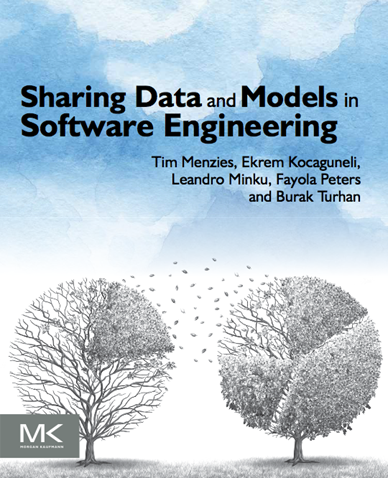
\includegraphics[width=1.45in]{fig/book1.png}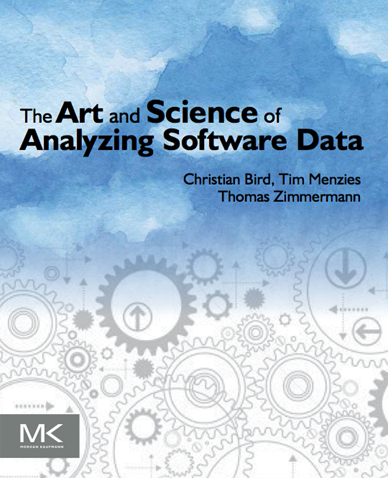
\includegraphics[width=1.45in]{fig/book2.png}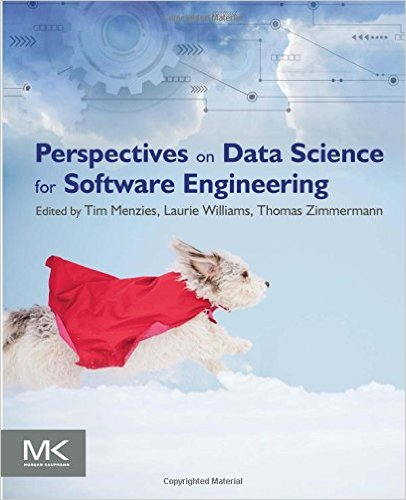
\includegraphics[width=1.45in]{fig/book3.jpg}
\caption{PI Menzies has co-written    three textbooks about 
empirical SE~\cite{menzies2014sharing,bird2015art,menzies2016perspectives}. But is any of that work relevant to
 computational science?}\label{fig:books}
\end{wrapfigure}

Many high-stake applications such as finance, hiring, admissions, criminal justice use algorithmic decision-making frequently. In some cases, machine learning models make better decisions than human can do \cite{Brun:2018:SF:3236024.3264838,Aydemir:2018:RES:3194770.3194778}. But there are many scenarios where machine learning software has been found to be biased and generating arguably unfair decisions. Google's sentiment analyzer model which determines positive or negative sentiment, gives negative score to the sentences such as \textit{`I am a Jew', and `I am homosexual'}\cite{Google_Sentiment}. Facial recognition software which predicts characteristics such as gender, age from images has been found to have a much higher error rate for dark-skinned women compared to light-skinned men \cite{Gender_Bias}. A popular photo tagging model has assigned animal category labels to dark skinned people \cite{Google_Photo}. Recidivism assessment models used by the criminal justice system have been found to be more likely to falsely label black defendants as future criminals at almost twice the rate as white defendants \cite{Machine_Bias}. Amazon.com stopped using automated job recruiting model after detection of bias against women\cite{Amazon_Bias}. Cathy O'Neil provided even more examples of unfair decisions made by software in her book ``Weapons of Math Destruction''\cite{O'Neil:2016:WMD:3002861}. She argued that machine learning software generates models that are full of bias. Hence, this is one of the reasons their application results in unfair decisions.


Machine learning software, by its nature, is always a form of statistical discrimination. The discrimination becomes objectionable when it places certain privileged groups at systematic advantage and certain unprivileged groups at systematic disadvantage. In certain situations, such as employment (hiring and firing), discrimination is not only objectionable, but illegal.


Issues of \textit{fairness} have been explored in many  recent papers in the SE research literature. Angell et al. \cite{Angell:2018:TAT:3236024.3264590}  commented that issues of fairness are analogous to other measures of software quality. Galhotra and his colleagues discussed how to efficiently generate test cases to test for discrimination\cite{Galhotra_2017}. Udeshi et al. \cite{Udeshi_2018} worked on generating discriminatory  inputs for machine learning software. Albarghouthi et al. \cite{Albarghouthi:2019:FP:3287560.3287588} explored if fairness can be wired into annotations within a program while Tramer et al. proposed different ways to measure discrimination \cite{Tramer_2017}.

All the above SE research detects unfairness. Our work takes a step further and asks how to mitigate
unfairness. We propose that every machine learning model must go through fairness testing phase before it is applied. If bias is found, then the model needs to be optimized. Hence, we have converted ``discrimination problem'' into an optimization problem. We think that if \textit{fairness} becomes a goal while learning, then the  models created in that way will generate fairer results. In this study, we investigated whether model parameter tuning can help us to make the model fair or not. 
 
 In machine learning, many  {\em hyperparameters} control   inductive process ; e.g. the   `splitter' of CART~\cite{breiman2017classification}.  They are very important because they directly control the behaviors of the training algorithm and impact the performance of the model. Therefore, the selection of appropriate parameters plays a critical role in the performance of machine learning models. Our study applies \textit{hyperparameter optimization} to make a model fair without losing predictive power. So, it becomes \textit{multiobjective optimization} problem as we are dealing with more than one objective. 
 
 \begin{table}[]
\centering
\scriptsize
\caption{Optimizing just for fairness.  
Change in  Recall and False alarm before and after bias mitigation. Gray= improvement; black= damage.}
\label{tbl:fairness_cost}
\begin{tabular}{|l|c|c|r|r|r|r|}
\hline
\rowcolor[HTML]{C0C0C0} 
\cellcolor[HTML]{C0C0C0} & \multicolumn{1}{l|}{\cellcolor[HTML]{C0C0C0}} & \multicolumn{1}{l|}{\cellcolor[HTML]{C0C0C0}} & \multicolumn{2}{c|}{\cellcolor[HTML]{C0C0C0}Recall} & \multicolumn{2}{c|}{\cellcolor[HTML]{C0C0C0}False alarm} \\ \cline{4-7} 
\rowcolor[HTML]{C0C0C0} 
\multirow{-2}{*}{\cellcolor[HTML]{C0C0C0}Algorithm} & \multicolumn{1}{l|}{\multirow{-2}{*}{\cellcolor[HTML]{C0C0C0}Dataset}} & \multicolumn{1}{l|}{\multirow{-2}{*}{\cellcolor[HTML]{C0C0C0}\begin{tabular}[c]{@{}l@{}}Protected \\ Attribute\end{tabular}}} & \multicolumn{1}{c|}{\cellcolor[HTML]{C0C0C0}Before} & \multicolumn{1}{l|}{\cellcolor[HTML]{C0C0C0}After} & \multicolumn{1}{c|}{\cellcolor[HTML]{C0C0C0}Before} & \multicolumn{1}{l|}{\cellcolor[HTML]{C0C0C0}After} \\ \hline
\multicolumn{1}{|c|}{} &  & Sex & 0.83 & \cellcolor[HTML]{FFFFFF}{\color[HTML]{333333} 0.83} & 0.34 & \cellcolor[HTML]{333333}{\color[HTML]{FFFFFF} 0.43} \\ \cline{3-7} 
\multicolumn{1}{|c|}{} & \multirow{-2}{*}{Adult} & Race & 0.83 & \cellcolor[HTML]{FFFFFF}{\color[HTML]{333333} 0.83} & 0.34 & \cellcolor[HTML]{333333}{\color[HTML]{FFFFFF} 0.35} \\ \cline{2-7} 
\multicolumn{1}{|c|}{} &  & Sex & 0.60 & 0.60 & \cellcolor[HTML]{FFFFFF}{\color[HTML]{333333} 0.27} & \cellcolor[HTML]{333333}{\color[HTML]{FFFFFF} 0.29} \\ \cline{3-7} 
\multicolumn{1}{|c|}{} & \multirow{-2}{*}{Compas} & Race & 0.62 & \cellcolor[HTML]{333333}{\color[HTML]{FFFFFF} 0.61} & \cellcolor[HTML]{FFFFFF}{\color[HTML]{333333} 0.27} & \cellcolor[HTML]{333333}{\color[HTML]{FFFFFF} 0.34} \\ \cline{2-7} 
\multicolumn{1}{|c|}{} &  & Sex & 0.70 & \cellcolor[HTML]{333333}{\color[HTML]{FFFFFF} 0.69} & \cellcolor[HTML]{FFFFFF}0.66 & \cellcolor[HTML]{333333}{\color[HTML]{FFFFFF} 0.77} \\ \cline{3-7} 
\multicolumn{1}{|c|}{\multirow{-6}{*}{Reweighing}} & \multirow{-2}{*}{German} & Age & 0.70 & \cellcolor[HTML]{C0C0C0}0.71 & \cellcolor[HTML]{FFFFFF}0.66 & \cellcolor[HTML]{C0C0C0}0.25 \\ \hline
 &  & Sex & 0.83 & \cellcolor[HTML]{333333}{\color[HTML]{FFFFFF} 0.76} & \cellcolor[HTML]{FFFFFF}0.34 & \cellcolor[HTML]{333333}{\color[HTML]{FFFFFF} 0.35} \\ \cline{3-7} 
 & \multirow{-2}{*}{Adult} & Race & 0.83 & 0.83 & \cellcolor[HTML]{FFFFFF}0.34 & \cellcolor[HTML]{333333}{\color[HTML]{FFFFFF} 0.37} \\ \cline{2-7} 
 &  & Sex & 0.60 & 0.60 & \cellcolor[HTML]{FFFFFF}0.27 & \cellcolor[HTML]{333333}{\color[HTML]{FFFFFF} 0.29} \\ \cline{3-7} 
 & \multirow{-2}{*}{Compas} & Race & 0.62 & \cellcolor[HTML]{C0C0C0}{\color[HTML]{333333} 0.65} & \cellcolor[HTML]{FFFFFF}0.27 & \cellcolor[HTML]{333333}{\color[HTML]{FFFFFF} 0.29} \\ \cline{2-7} 
 &  & Sex & 0.70 & \cellcolor[HTML]{333333}{\color[HTML]{FFFFFF} 0.69} & \cellcolor[HTML]{FFFFFF}0.66 & \cellcolor[HTML]{C0C0C0}{\color[HTML]{333333} 0.36} \\ \cline{3-7} 
\multirow{-6}{*}{\begin{tabular}[c]{@{}l@{}}Optimized \\ Pre-\\ processing\end{tabular}} & \multirow{-2}{*}{German} & Age & 0.70 & \cellcolor[HTML]{333333}{\color[HTML]{FFFFFF} 0.68} & \cellcolor[HTML]{FFFFFF}0.66 & \cellcolor[HTML]{C0C0C0}{\color[HTML]{333333} 0.58} \\ \hline
 &  & Sex & 0.82 & \cellcolor[HTML]{C0C0C0}0.83 & 0.35 & \cellcolor[HTML]{333333}{\color[HTML]{FFFFFF} 0.42} \\ \cline{3-7} 
 & \multirow{-2}{*}{Adult} & Race & 0.82 & 0.82 & 0.35 & 0.35 \\ \cline{2-7} 
 &  & Sex & 0.60 & 0.60 & 0.27 & \cellcolor[HTML]{333333}{\color[HTML]{FFFFFF} 0.28} \\ \cline{3-7} 
 & \multirow{-2}{*}{Compas} & Race & 0.60 & 0.60 & 0.27 & \cellcolor[HTML]{333333}{\color[HTML]{FFFFFF} 0.28} \\ \cline{2-7} 
 &  & Sex & 0.70 & \cellcolor[HTML]{C0C0C0}0.75 & 0.66 & \cellcolor[HTML]{C0C0C0}0.61 \\ \cline{3-7} 
\multirow{-6}{*}{\begin{tabular}[c]{@{}l@{}}Adversial\\ Debiasing\end{tabular}} & \multirow{-2}{*}{German} & Age & 0.70 & \cellcolor[HTML]{333333}{\color[HTML]{FFFFFF} 0.69} & 0.50 & \cellcolor[HTML]{333333}{\color[HTML]{FFFFFF} 0.72} \\ \hline
 &  & Sex & 0.83 & \cellcolor[HTML]{333333}{\color[HTML]{FFFFFF} 0.24} & 0.34 & \cellcolor[HTML]{C0C0C0}0.05 \\ \cline{3-7} 
 & \multirow{-2}{*}{Adult} & Race & 0.83 & \cellcolor[HTML]{333333}{\color[HTML]{FFFFFF} 0.28} & 0.34 & \cellcolor[HTML]{C0C0C0}0.04 \\ \cline{2-7} 
 &  & Sex & 0.62 & \cellcolor[HTML]{C0C0C0}{\color[HTML]{333333} 0.97} & 0.27 & \cellcolor[HTML]{333333}{\color[HTML]{FFFFFF} 0.89} \\ \cline{3-7} 
 & \multirow{-2}{*}{Compas} & Race & 0.62 & \cellcolor[HTML]{C0C0C0}{\color[HTML]{333333} 0.68} & 0.27 & \cellcolor[HTML]{333333}{\color[HTML]{FFFFFF} 0.38} \\ \cline{2-7} 
 &  & Sex & 0.70 & \cellcolor[HTML]{C0C0C0}{\color[HTML]{333333} 0.96} & 0.66 & \cellcolor[HTML]{333333}{\color[HTML]{FFFFFF} 0.95} \\ \cline{3-7} 
\multirow{-6}{*}{\begin{tabular}[c]{@{}l@{}}Reject\\ Option\end{tabular}} & \multirow{-2}{*}{German} & Age & 0.70 & 0.70 & 0.66 & 0.66 \\ \hline
 &  & Sex & 0.83 & \cellcolor[HTML]{333333}{\color[HTML]{FFFFFF} 0.78} & 0.39 & \cellcolor[HTML]{333333}{\color[HTML]{FFFFFF} 0.40} \\ \cline{3-7} 
 & \multirow{-2}{*}{Adult} & Race & 0.83 & \cellcolor[HTML]{333333}{\color[HTML]{FFFFFF} 0.78} & 0.39 & \cellcolor[HTML]{C0C0C0}0.35 \\ \cline{2-7} 
 &  & Sex & 0.65 & \cellcolor[HTML]{333333}{\color[HTML]{FFFFFF} 0.63} & 0.38 & \cellcolor[HTML]{333333}{\color[HTML]{FFFFFF} 0.40} \\ \cline{3-7} 
 & \multirow{-2}{*}{Compas} & Race & 0.65 & 0.65 & 0.38 & \cellcolor[HTML]{333333}{\color[HTML]{FFFFFF} 0.39} \\ \cline{2-7} 
 &  & Sex & 0.74 & \cellcolor[HTML]{333333}{\color[HTML]{FFFFFF} 0.72} & 0.20 & \cellcolor[HTML]{333333}{\color[HTML]{FFFFFF} 0.33} \\ \cline{3-7} 
\multirow{-6}{*}{\begin{tabular}[c]{@{}l@{}}FLASH\\ optimizes for\\ AOD \& EOD\end{tabular}} & \multirow{-2}{*}{German} & Age & 0.74 & \cellcolor[HTML]{333333}{\color[HTML]{FFFFFF} 0.68} & 0.20 & \cellcolor[HTML]{333333}{\color[HTML]{FFFFFF} 0.45} \\ \hline
\end{tabular}
\end{table}
 


\newpage
% Much recent empirical SE research has focused on this data, and how
% to leverage this kind of Github data to build software quality models~~\cite{commitguru, Kim08changes,catolino17_jitmobile,nayrolles18_clever,mockus00changeskeys,kamei12_jit,hindle08_largecommits}.

%  To simplify the creation and maintenance of computational science software, we   propose  the  {\IT}\footnote{ Short for 
% ``empirical \underline{SE} \underline{n}ow \underline{TRY}-ed on  computational science code''.} empirical software engineering workbench.
% {\IT} contains a set of automatic agents that read code and comments and test
% results from on-line repositories of computational science code.  {\IT} will advise:
% \bi
% \item[(a)] Where defects are hiding the code;
% \item[(b)] How to prioritize test cases (so tests  likely to fail are executed sooner); 
% \item[(c)] The appropriate number of programmers required
% for each project; 
% \item[(d)] Now to avoid spurious error messages (e.g. from static code analysis tools);
% \item[(e)] Other issues, if time permits.
% \ei
% While many parts of {\IT} have been proposed in other domains,
% results from a recent NSF EAGER grant, described below\footnote{CISE EAGER \#1826574.  Empirical Software Engineering for Computational Science. April 2018 to April 2019. PI= Tim Menzies.}, show that standard SE needs adaptation before it can succeed on computational
% science software. This proposal would explore cost-effective methods for managing that adaption process. The resulting agents
% will then be tested on all the   computational science projects currently available on the web (e.g. see the sample in  \tbl{samples}).
%  This, in turn, will enable faster and better  software development  leading to   faster and greater progress in computational science.
% \begin{table}
\caption{Initially,
this proposal will focus on the following
 samples of active computational science projects
(all of which are found in on-line open source repositories). 
{\normalfont Robert Sinkovits (from XSEDE) comments that many of these codes account for the majority of the supercomputer usage in computational
science. While some of these  focus on  computational chemistry,  they   also   include  numerous widely-used support tools (e.g
elasticsearch) or simulation tools that are cross-disciplinary (e.g. the classical simulation tools
used  by molecular biologists).  Also, there are also tools here used in material science (e.g. LAMMPS).
Further, these are just some of the projects found during an initial EAGER-funded projects so, during the three years of
this current proposal, we anticipate that many more projects will be discovered and analyzed by {\IT}.}
}\label{tbl:samples}
{\footnotesize
\begin{center}
\begin{tabular}{r|l@{~}rrr@{~}r@{~}r@{~}rrc}
\renewcommand{\baselinestretch}{0.7}
&   &   &   &   &  &  &   & Analyzed\\  
 & Language & \# Developers & Duration(Years) & \# Commits & \# Stars & \# Issues & \# Releases & in Figure~2\\ 
\hline
BLIS & C & 20 & 4.8 & 1242 & 413 & 142 & 25 &   \\ 
cctools & C	 & 43	& 5.5 & 8881	& 72 & 666 & 159  &   \\
keplerproject & C & 22	& 5.25 & 329 & 26 & 66	& 18 &   \\

\hline
\rowcolor{blue!10}AMBER & C++ & 12 & 4 & 8382 & 32 & 249 & 3 & \checkmark\\
changa & C++ & 19	& 3.5 & 1458 & 13 & 16 & 8 &   \\
cyclus & C++ & 20	& 6.5 & 6579 & 36 & 625	& 47 &   \\
dealii & C++ & 120 & 18 & 41514 & 382 & 1604 & 26 &   \\
GooFit & C++ &	12	& 5.5  & 1508	& 57 & 50	& 12 &   \\
\rowcolor{blue!10}HooMD-blue & C++ & 36 & 2.5 & 9450 & 54 & 330 & 25 & \checkmark \\
irods & C++	& 36 & 5 & 6267 & 236 & 3820 & 34 &   \\
\rowcolor{blue!10}LAMMPS & C++ & 74 & 5.13 & 15814 & 383 & 294 & 91 & \checkmark \\ 
\rowcolor{blue!10}LIBMESH & C++  & 55 & 6 & 17133 & 247 & 449 & 59 & \checkmark \\ 
MADNESS & C++ & 31 & 4.5 & 5193 & 71 & 184 & 3 &   \\
metpy & C++	& 34	& 7.75 & 2199 & 332 & 481 & 20 &   \\
OpenMm & C++ & 38 & 7 & 5838 & 324 & 959 & 22 &   \\
OpenMX & C++ & 11 & 5 & 6993 & 26 & 79 & 62 &   \\
\rowcolor{blue!10}PCMSolver & C++ & 8 & 4 & 1844 & 13 & 88 & 16 & \checkmark \\ 
PLUMED & C++ & 23 & 5.5 & 8075 & 92 & 282 & 35 &   \\
Psi4 & C++ & 79 & 5.5 & 12178 & 247 & 504 &	7 &   \\
SCIRun & C++ & 18	& 6.5 & 8887 & 45 & 1487 &79 &   \\
TRILINOS & C++ & 179 & 3 &	79520 & 310  &	2063 &	141 &   \\\hline
  \rowcolor{blue!10}ABINIT  & Fortran & 23 & 2.3 & 6793 & 53 & 13 & 96 & \checkmark  \\ 
 OpenMolcas & Fortran & 29 & 1 & 565 & 29 & 52 & 2 &   \\ 
MPQC & C++, Fortran & 12 & 5 & 6362 & 28 & 44 & 57 &   \\
NWChem & Fortran & 29 & 1 & 26013 & 70 & 33 & 5 &   \\
OpenMPI & C, Fortran & 147 & 4 &	28680 & 627 & 1424  & 99 &   \\
quantum\_package & Fortran & 11 & 4.5 & 2721 & 18 & 92 & 5 &   \\\hline
elasticsearch & Java & 1103 & 8.5 & 42349 & 37757 & 16918 & 223 &   \\
learnsphere & Java &  9 & 2.5 & 646	& 11 & 34 & 1 &   \\
orca & Java	& 11 & 3.5 & 1103 & 1 & 143	& 19 &   \\
trellis & Java & 3 & 2 & 892 & 26 & 171 & 10 &   \\
\rowcolor{blue!10}Xenon & Java  & 11 & 9 & 2315 & 15 & 378 & 21 & \checkmark \\\hline
abaco & Python 	& 8	& 3.5 & 1112 & 13 & 29 & 7 &   \\
APBS & Python & 19 & 5 & 6642 & 67 & 501 & 8 &   \\
forcebalance & Python &	10 & 5 & 1562 & 48 & 47 &	6 &   \\
foyer & Python & 10 & 3.5 &	343 & 19 &	66 & 8 &   \\
hydroshare & Python	& 30 & 4 &	9387 & 63 & 1708	& 55 &   \\
Luigi & Python & 35 & 6 & 3628 & 10348 & 628	& 37 &   \\
mast & Python & 22	& 5.5 & 5050 & 8 & 471	& 69 &   \\
\rowcolor{blue!10} MDAnalysis & Python & 76 & 3.5 & 5120 & 233 & 1087 & 46 & \checkmark \\
mdtraj & Python	& 45	& 6 & 2971 & 189 & 682	& 21 &   \\
openforcefield & Python &	8	& 1 &1360 & 37	& 70	& 5 &   \\
openmmtools & Python &	10 & 4 &	1156 & 40  & 154	& 31 &   \\
parsl & Python & 11	& 2 & 1268 & 63 & 258	& 15 &   \\
pymatgen & Python & 107	& 7 & 14989	& 322 & 359	& 228 &   \\
pyscf & Python	& 36 & 4.5 & 4666 & 217 & 101	& 41 &   \\
radical-pilot & Python & 17	&  5 & 56900 & 26 & 1269 & 137 &   \\
\rowcolor{blue!10} RMG-Py & Python  & 43 & 1 & 7548 & 112 & 678 & 17 & \checkmark \\
signac & Python	& 8	& 2 & 5000 & 8	& 89 &	5 &   \\
signac-flow & Python &	8 & 2 & 1000 & 5 & 28	&3 &   \\
TauDEM & Python	& 11 & 5.5 & 298 & 102 & 132 & 10 &   \\
Use Galaxy & Python	& 188 & 3.5 & 36005 & 507 & 2269 & 51 &   \\
yank & Python &	8 & 5  &	2728 & 41 & 557 & 34 &   \\
yt & Python & 93 & 1.5 & 23923 & 138 & 1216 & 37 &   \\

\end{tabular}\end{center}}
\label{tbl:summary}
\end{table}




 
% Standard methods in empirical software engineering (SE) needs to be adapted before it can be safely deployed in other
% domains like computational science (see below, example in defect prediction). But what adaption methods are useful/useless? Are
% they cost effective? Do they work effectively across multiple data sets? We have some preliminary results suggesting that the work
% for (a) defect prediction but can we also adapt other tasks such as (b) test case prioritization, (c) effort estimation, (d) learning to
% avoid spurious error message; (e) etc.





\section{Frequently Asked Questions}\label{tion:faq}
{\em Q1: Does software discrimination(bias towards certain attribute) matters?}

Yes.Google's sentiment analyzer model which determines positive or negative sentiment, gives negative score to the sentences such as \textit{`I am a Jew', and `I am homosexual'}\cite{Google_Sentiment}. Facial recognition software which predicts characteristics such as gender, age from images has been found to have a much higher error rate for dark-skinned women compared to light-skinned men \cite{Gender_Bias}. A popular photo tagging model has assigned animal category labels to dark skinned people \cite{Google_Photo}. Recidivism assessment models used by the criminal justice system have been found to be more likely to falsely label black defendants as future criminals at almost twice the rate as white defendants \cite{Machine_Bias}. Amazon.com stopped using automated job recruiting model after detection of bias against women\cite{Amazon_Bias}. Cathy O'Neil’ provided even more examples of unfair decisions made by software in her book ``Weapons of Math Destruction''\cite{O'Neil:2016:WMD:3002861}. She argued that machine learning software generates models that are full of bias. Hence, this is one of the reasons their application results in unfair decisions.

{\em Q2: Does certain attributes(protected) creates software  discrimination in prediction results ?}

Yes.

{\em Q3: Does removing above mentioned protected attribute have effect on model's performance ?}

Yes

{\em Q4: Does optimizing for fairness damage model prediction performance ?}

No. We have verified our method along with four other related works to answer this question. Table \ref{tbl:dataset} shows the datasets we used. We randomly divided them into three sets - training (70\%), validation (15\%) and test (15\%). Prior researchers who worked with these datasets have used \textit{Logistic Regression} as classification model \cite{Kamishima,NIPS2017_6988,Hardt}. We also decided to use this learner. Before moving to results, here we briefly describe prior works which we selected for our study. There are mainly three kinds of prior works -

\bi
\item \textbf{Pre-processing algorithms}: In this method, data is pre-processed(before classification) in such a way that discrimination is reduced. Kamiran et al. proposed \textit{Reweighing} \cite{Kamiran2012} method that generates weights for the training examples in each (group, label) combination differently to ensure fairness. Later, Calmon et al. proposed an \textit{Optimized pre-processing} method \cite{NIPS2017_6988} which learns a probabilistic transformation that edits the labels and features with individual distortion and group fairness.


\item \textbf{In-processing algorithms}: This is an optimization approach where dataset is divided into train, validation and test set. After learning from training data, model is optimized on the validation set and finally applied on the test set. Our \textit{Hyperparameter Optimization} using FLASH approach lies into this category. Zhang et al. proposed \textit{Adversarial debiasing}  \cite{Zhang:2018:MUB:3278721.3278779} method which learns a classifier to maximize accuracy and simultaneously reduce an adversary's ability to determine the protected attribute from the predictions. This generates a fair classifier because the predictions cannot carry any group discrimination information that the adversary can exploit.


\item \textbf{Post-processing algorithms}: Hereafter classification, the class labels are changed to reduce discrimination. Kamiran et al. proposed \textit{Reject option classification} approach \cite{Kamiran:2018:ERO:3165328.3165686} which gives unfavorable outcomes to privileged groups and favorable outcomes to unprivileged groups within a confidence band around the decision boundary with the highest uncertainty.

\ei

Table \ref{tbl:fairness_cost} shows the results of our approach (FLASH) and four algorithms from prior works. We see that there are a few gray cells and many black cells indicating that achieving fairness damages performance - which bolsters the conclusion made by Berk et al.\cite{berk2017convex}. In summary,  fairness can have a cost. Our next question checks if multiobjective optimization can better trade-off between performance and fairness.  

{\em Q5: Can we optimize machine learning model for both fairness and performance?}

Yes. Here, we applied  FLASH algorithm but this time, we considered four goals together: \textit{recall, false alarm, AOD, EOD}. The first two are related to performance and second two are related to fairness. For
recall, {\em larger} values are {\em better} while for everything
else, {\em smaller} is {\em better}.
 For this part of our study, we used two learning models - logistic regression and CART. 
 %Afer a model is learnrf from the training set. On the validation set, the model is tuned and recall, false alarm, AOD \& EOD are noted down when tuned learner is applied on the test set.
 
 We have chosen four hyperparameters for both the learners to optimize for. For logistic regression (C, penalty, solver, max\_iter) and for CART - (criterion, splitter , min\_samples\_leaf, min\_samples\_split). Table \ref{tbl:multiobjective_results} shows the results. The ``Before'' column shows results with no tuning and ``After'' column shows tuned results. We can see that for
 the German dataset, we improved three objectives and recall did not decrease. In the Adult dataset, we improved three objectives with minor damage of recall. 
 With the
 Compas dataset, there was no improvement. 
 
 In summary, the results are clearly indicating if  multiobjective  optimization understand {\em all} the goals of learning
 (fairness {\em and performance}), then it is possible to achieve one without
 damaging the other. Our last research question asks  what is the cost of this kind of optimization.

{\em Q6. How much time does optimization take?}

Default logistic regression takes 0.56s, 0.15s and 0.11s for Adult, Compas and German dataset respectively. When we apply hyperparameter optimization, the cumulative time for training, tuning and testing become 16.33s, 4.34s and 3.55s for those datasets. 
We assert that  runtimes of less than 20 seconds is a relatively small price to pay to ensure fairness. 

As to larger, more complex problems, Nair et al.~\cite{8469102} reports
that FLASH scales to problems with larger order of magnitude than other optimizers. It is a matter for future research to see if such scale is possible/required to handle fairness of SE data. 




\section{ Technical Details}\label{tion:details}



The rest of this proposal offers details  on the 
\underline{S}trategies, \underline{En}deavors, 
\underline{T}uners,
inst\underline{R}uments and \underline{Y}ields
that will implemented and explored as part
of the {\IT} workbench. 

\subsection{Target Endeavors}\label{tion:ende}

Recall that {\IT} is intended to reduce the
time required to handle  many  tedious,
aspects of software development, thereby  freeing up the time of computational scientists to think
more about core scientific issues. This proposaal will explore
several  such tasks:
\bi
\item[(a)] 
{\em Manually reviewing code} which we will optimize with defect predictors that tell developers where to look first to find most bugs (see \tion{dp}).
\item[(b)] {\em Running large test suites}
which we will optimize with test case prioritization
strategies that {\em first} run the tests
most likely to fail  sooner (thus allowing developers to stop long test run, sooner, once they acquire   enough issues to fix)
(see \tion{test}).
\item[(c)]  {\em Deciding what issues to act on  and which to 
ignore} which we will optimize with 
active learning tools that learn which are the important warnings that must be fixed
(see \tion{falsealarm}).
\item [(d)] {\em Managing programming projects}
which we will optimizer with technical debt detectors
that can advise when there are too many, or not enough, programmers working on software
(see \tion{effort}).
\item[(e)] And other tasks, as time and opportunity permits and as requested by   computational
scientists.
\ei
These tasks were selected since, as discussed below, there is much research research on all the above in the empirical SE literature. Hence they serve to check if the concerns of standard
empirical SE can serve the computational science community.
 
 \subsection{Practicality}\label{tion:practical}

\begin{wrapfigure}{r}{3in}
\vspace{-5mm}
\begin{center}
{\small
\begin{tabular}{c|c|ccc} 
 \multicolumn{1}{c}{{\bf Endeavor }}&Section &{\em dm }& {\em ho}& {\em al  } \\\hline 
defect prediction   &\tion{dp}    &     \checkmark         &          \checkmark               &       \checkmark                  \\  
test case prioritization& \tion{test} &    \checkmark          &     \checkmark                 &     \checkmark                   \\
handling warnings     & \tion{falsealarm} &    \checkmark          &                       &        \checkmark                  \\
technical debt        & \tion{effort}  &     \checkmark          &    \checkmark                   &   \checkmark                        \\

\end{tabular}}
\end{center}
\caption{{\bf Strategies} for {\bf tuning} the {\bf instruments} of different {\bf endeavors}.
Column titles {\em dm, ho, al} are explained later in this proposal. }
\label{tbl:reuse}
\vspace{-20mm}
\end{wrapfigure}
It is prudent to consider the practicality of exploring
all of the (a)(b)(c)(d)(e) endeavors from \tion{ende}. Is this list too long for
one NSF project? We think not and   \tbl{reuse} explains why.

This table shows   some of the software tools
to used in this work. 
The column names describe different {\bf strategies} that are explained later in this proposal:
\bi
\item {\em dm} = data miners; 
\item {\em ho} = hyperparameter optimization;
\item {\em al} = active learning.
\ei
Our experience is that,
when used together, this triad of {\bf strategies}
offers a general framework for commissioning
empirical SE to new domains. In support  of
the last sentence,  we note that:
\bi
\item When there is too much data to look at,
{\em data miners} can automatically find important patterns.
\item When there are too many options about how
to configure a data miner, 
{\em hyperparameter optimizers} can automatically find the best settings.
\item 
When it is too expensive to check all the results
from data mining and hyperparameter optimization,
{\em active learners} can prune away the uninformative examples, leaving behind  a manageably
small number of examples to check.
\ei
More importantly, this triad
of {\bf strategies} can be reused
in multiple {\bf endeavors} (as seen in \tbl{reuse}).  That is, 
once one endeavor is completed, we will have much of the infrastructure needed for the next endeavor.
Hence we are confident that  this grant,
we can explore the {\bf endeavors}  (a)(b)(c)(d)(e) 
listed in  \tion{ende}.



\subsection{About Four Different Endeavors}\label{tion:four}
This proposal will explore  four
{\bf endeavors} (described in this section)
in order to 
to collect the data needed to test the  Claims 1,2,3,4,5 made in the introduction. 


Anyone  interested in the ``how'', rather than the ``what'', of this project
might care to skip to the Management Plan on page \pageref{tion:plan}. That section 
 describes how  data
will be collected  and used
to test Claims 1,2,3,4,5.  The key thing to note
there is that many of those
tests will need to know how to measure
the {\bf yield} of different {\bf endeavors}:
\bi
\item As discussed in \tion{dp}, the {\bf yields} for {\em defect prediction} are many and varied and include measures such as \eq{ostrand} (where  {\em larger} values are {\em better}).
\item 
As discussed in \tion{test},
the {\bf yield} for
{\em test case prioritization}
is the  time taken to find X\% of the failing tests, expressed as a ratio of the time required by a ``perfect'' oracle (so {\em larger} values are {\em better}).
\item 
As discussed in \tion{falsealarm},
the {\bf yield} for {\em learning to avoid
spurious warnings} is how few warnings have to be inspected before a classifier can be learned to 
assess the remaining warnings (so here, {\em faster} learning time is {\em better}).
\item As discussed in \tion{effort},  two {\bf yields} for
{\em technical debt 
management} are (a) how quickly
can we learn to recognize programmer comments
indicate technical debt (so {\em faster} values are {\em better}); and (b)
 how well can we recognize when the
projects are encouraging technical debt
via  a suspiciously low number of developers
(so {\em smaller} errors in estimating the required number of developers  are {\em better}).
\ei







\subsubsection{Endeavoring to   Predict Defects}\label{tion:dp}

% As soon as people started programming, it became apparent
% that programming was an inherently buggy process. As recalled
% by Maurice Wilkes~\cite{wilkes1985memoirs}, speaking of his programming experiences from the early 1950s: ``It was on one of my journeys between the EDSAC room and the punching equipment that `hesitating at the angles of stairs' the realization came over me with full force that a good part of the remainder of my life was going to be spent in finding errors in my own programs.''
This section describes the defect prediction task explored in Figure~2.
As mentioned in the introduction, the Figure~2 results are somewhat limited (less than a dozen projects) so for this new proposal we would test the generality
of the Figure~2 results (by exploring data from many more projects).
 
 Research shows
that software bugs are not distributed evenly across
a system. Rather, they seem to clump in small corners of the code. For example,
Hamill et al.~\cite{hamill09} report studies with the GNU C++ compiler
where half of the files were never implicated in issue reports while 10\% of
the files were mentioned in half of the issues. Also,
Ostrand et al.~\cite{Ostrand:2004} studied
AT\&T data and reported that 80\% of the bugs reside in 20\% of the files.
Further, a similar ``80-20'' patterns have been seen in NASA systems~\cite{hamill09};
open-source software~\cite{koru2009investigation}; and software
from Turkey~\cite{misirli2011ai}. 

Given this skewed distribution,  a
cost-effective   quality assurance approach is required to  sample
across a   system, then focus  on regions reporting some
bugs.
Software defect predictors built from data miners are 
 one way to implement such a sampling policy.   Their conclusions
are never 100\% correct, but they can  suggest where to focus more expensive  methods such as elaborate manual
review of source code~\cite{Shull:2001}; symbolic execution checking~\cite{paaareanu2008combining}, etc.
 Misirli et al.~\cite{misirli2011ai} found that  the guidance offered by
defect predictors
significantly reduced  
software inspection effort (by 72\%) in  Turkish software companies 
while still     letting them to localize
their faults (find the  25\% of the files that
have 88\% of the defects).

% Not only do static code defect predictors perform well compared to manual methods,
% they also are competitive with certain automatic methods.
% A recent study at ICSE'14, Rahman et al.~\cite{rahman2014comparing} compared
% (a) static code analysis tools FindBugs, Jlint, and Pmd and (b)
% static code defect predictors
% (which they called ``statistical defect prediction'') built using logistic regression.
% They found  no significant differences in the cost-effectiveness
% of these  approaches. Given this equivalence, it is significant to note that 
% static code defect prediction can be quickly adapted to new languages by building lightweight
% parsers that extract static code metrics. The same is not true for   static code analyzers-- these need  extensive modification before they can be used on new
% languages.

{\IT} will implement code to assess
defect prediction  {\bf yield} in multiple ways
since,
in our experience,
it is best  evaluate defect predictors on multiple {\bf yield}s.
(Why? Because it is possible to succeed according
to one   {\bf yield}   (e.g., recall)
while failing on another (e.g. false alarm)~\cite{fu2016tuning}). Also,
we deprecate the use of  precision and accuracy since these can be misleading for imbalanced data sets where the target class is somewhat
rare ~\cite{Menzies:2007prec}. 
In other research, Ostrand proposes maximizing the ratio:
\begin{equation}\label{eq:ostrand}P\;/\;L\end{equation}
where $P$ is the percent of bugs found after reading  $L$ lines~\cite{Ostrand:2004}. In this
expression, maximum
{\bf yield} come from finding the most bugs after reading the fewest lines of code. 
For lists of different ways to measure {\bf yield}, see table 23.2 of~\cite{menzies2014sharing} and Section~5 of~\cite{lo17_ifa}. All these will be implemented in {\IT}.

{\IT} will include
 many {\bf instruments} for  defect prediction.
 For example, we will include all the machine learning algorithms
studied by Ghotra'15~\cite{Ghotra15}.
We will also include the data pre-processing methods endorse
by Agrawal etl'18~\cite{agrawal2017better},
which includes methods for class frequency re-balancing.
Further, 
we will integrate with  Commit.Guru~\cite{commitguru},
thus enabling  
web-scale data collection. Lastly,
we will use  the SZZ algorithm to find
what code lead to bug reports~\cite{costa17szz, Kim08changes, Sliwerski05changes,RODRIGUEZPEREZ2018164}.

Figure~2 reported our experience applying   standard SE {\bf instruments}
to computational science.
The lesson learned from that work was
that, before {\IT} could work for
computational science, we had to {\bf tune} those methods. 
There are many ways to {\bf tune} defect predictors:
\bi
\item Adjust creation of  {\em dependent variables} to  better handled (e.g.) 
class labelling ~\cite{commitguru} or class imbalance~\cite{agrawal2017better};
or (e.g.) generate better initial labels (as done in Figure~2).
\item Adjust creation of    {\em independent variables} via better 
descritization~\cite{fayyad1993multi,Dougherty:1995} or feature selection~\cite{menzies07w,hall2003benchmarking};
\item Adjust the control settings of the learner which,
in turn, adjusts how the {\em independent} variables are combined together to predict
for the {\em dependent variables}~\cite{%
Agrawal19,%
fu2016tuning,%
nair2017flash,%
agrawal2017better}.
\item
After building defect predictors, it is possible
to reflect on the learned models to infer {\em guidelines }for how to decrease defects in future projects~\cite{xtree17}.
We make no causal claim there (e.g. that changing XYZ will definitely  reduce defects). Rather, these guidelines are more probabilistic statements that (e.g.)  the historical record 
shows  that Java methods with less than X lines  of code have least defects.
\ei
The above list shows {\em what}   can be tuned. The following list of {\bf strategies} shows {\em how} we might tune them:
 \bi

\item {\em Active learners} can help orchestrate a human+AI partnership~\cite{Cormack2017Navigating,Cormack2016Engineering,cormack2016scalability,Cormack2015Autonomy,cormack2014evaluation,grossman2013,wallace2010semi,wallace2010active,wallace2011should,wallace2012class,wallace2013active,Yu:2018,Yu2019}.
In this approach, humans watch over the conclusions made by an AI, sometimes
adjusting   faulty conclusions. AI then uses the conclusions to date to
select the next most informative example to show to humans.
For example, in Figure~2, our active learner was  an incremental SVM that reflected
on the support vectors to select the next commit message
to label ``buggy'' or ``not buggy''.
That active learning  
(a)~greatly reducing
the effort required by humans to review the conclusions of the AI
while (b)~also greatly increasing
the {\bf yield}  of the defect predictor (see the  \textcolor{ForestGreen}{\bf GREEN} triangles
of  Figure~2).
\item {\em Hyperparameter optimziation}  
 is the process of automatically searching the space of possible learners and their possible control settings. Such optimizers select learners/settings
in order to improve the {\bf yields} that are relevant to a particular project. Without such optimizers, it is something of a black-art to select the best learners/control settings. With those optimizers, it is possible to dramatically improve learner performance~\cite{agrawal2017better,fu2016tuning,tanti16defect,majumder2018}. State of the art hyperparameter optimizers include SMAC~\cite{Hutter:2011} and Hyperband~\cite{Li:2017}
and the FLASH algorithm~\cite{nair2017flash}  by Nair and
PI Menzies.
% \item  {\em Goal-aware data miners} 
% like WHICH~\cite{menzies2010defect} or FFTs~\cite{chen2018applications} or GA-based rule learners~\cite{Fernandez10,bacardit2013large,GARCIAPIQUER201769}   
% adjust the specifics of their internal
% search in order to match the users' desired {\bf yields}. For example, a standard learner would try to 
% accurately report potential defects.  But for developers with limited time, a better way to measure the {\bf yields} in terms of \eq{ostrand}.
\ei
It is an open empirical issue
which of these work best for  computational science
(hence, this proposal).
% That said, preliminary
% results are promising:
% \bi
% \item
% As reported above,
% the final analysis of Figure~2 took just a few weeks (once we had debugged our scripts)
% and was achieved with \$0 open source tools using standard desktop machines. 
% \item
% Active learning is  surprisingly general and can be applied to  many endeavors.
% We have preliminary results showing one active learner 
% (the one used for
% defect prediction in Figure~2) also works for endeavors such as 
% detecting software security vulnerabilities~\cite{Yu20},
% test case prioritization~\cite{zhu19b}, technical debt management~\cite{xia19},   and
% learning to avoid spurious warning messages~\cite{yang19b}.
% \item
% Hyperparameter optimization   can automate     an exploration of a large space
% of options.  
%  PI Menzies has    shown that  by exploiting 
%  data symmetries found in    data from software 
% projects, hyperparameter optimization can speed up
% by several orders of magnitude~\cite{%
% Agrawal19,%
% fu2016tuning,% 
% nair2017flash,%
% agrawal2017better,chen2017beyond,nair2016accidental,agrawal2016wrong}.

% % \item
% % To be sure, some goal-aware learning methods may be  complex and require hardware support in order
% % terminate in a reasonable time (e.g. large cloud-based CPU farms~\cite{bacardit2013large}. However, PI Menzies has found that for SE data,
% % if the discretization policy is informed by the desired {\bf yields}, then very simple rule learners can 
% % perform very well~\cite{menzies2010defect,chen2018applications}. For example, a standard discretization
% % method is to  divide numeric ranges to decrease class variance~\cite{Breiman1996}. But for SE
% % data, effective goal-aware learning can be achieved by discretizing numerics to maximize \eq{ostrand}.
% \ei
% That said, just to 
% say the obvious, we need to test
% if it is just as  practical 
% to apply empirical SE to computational science
%  using more projects
% and more endeavors (hence, this proposal).



\subsubsection{Endeavoring to Prioritize Test  Cases}\label{tion:test}
Defect prediction methods help members of one software team review their code.
Hence, it supports a {\em micro task} that occurs often deep within a software development project.

Test case prioritization, on the other hand,  is a {\em macro task} that struggles to tame the complexity of large scale testing.
 Test suite execution
is the rate determining step in software development (since faster
tests means faster delivery of  software to users).


 
Testing takes much of the time of modern software development. There are many reasons for this.
Firstly,
re-running all the tests is  important when communities work together on a single code
base. In that case, the polite (or cautious)  developer re-runs all the tests {\em before} she commits her code to the shared repository, just to ensure that their
changes will not introduce errors into the work of other people.
Secondly,  
experienced developers know how to write just enough code (and no more) to meet some requirement.
In
TDD~\cite{beck2003test} or ``test-driven development'',
 \textcolor{red}{\em red} tests (which always fail)
are written first. 
Next, developers write just enough code to make the tests turn  \textcolor{ForestGreen}{\em green} (i.e. pass). Also, sometimes,
developers  might refactor (i.e. reorganize) the code using  experience gained
from running the system. This cycle of \textcolor{red}{red}-\textcolor{ForestGreen}{green}-refactor is a widely-adopted practice
of agile programming. 
Thirdly, 
 TDD is  useful when prototoyping software
since it ensures that a test suite is built alongside the code base.
When prototyping,  the wise developer incrementally makes
small changes to the code then re-runs all the tests, just to ensure that their most recent changes are not damaging the code base. Observe that when prototyping with TDD, developers are 
constantly re-running their tests.


Elbaum et al~\cite{google} recently showed how to faster find failing tests. That work explored the Google test case prioritization problem. Google developers were advocates of TDD and so, as part of their
code, there were many tests.
Hence, between January and October 2013, Google ran three billion unit tests. In that suite,
it was taking days before any failing tests were found. Elbaum et al.
found that by  weighing tests by 
how long since they last failed;
how new were the tests;
and how long since they were last executed;
then  many of their tests started failing much faster (sometimes, even within an hour). 

\newpage

\begin{table}[!t]
\caption{A Sample of Test Case Prioritization {\bf Strategies}.
}
\label{tbl:algorithms}
\resizebox{\textwidth}{!}{
\small
\setlength\tabcolsep{5pt}
\begin{tabular}{cl|ccc|}
\multicolumn{2}{c|}{~}                & \multicolumn{3}{c|}{\textbf{Utilized Information}}\\ 
\multicolumn{2}{c|}{~}      & Execution      & Test case        &         \\ 

\textbf{ID}     & \textbf{Algorithm Description}       &  history     &   description       & Feedback       \\ \hline
\rowcolor{blue!10} A1 & Regression testing in random order. & & &  \\ 
\rowcolor{blue!10}  A2 & Regression testing in optimal order. & & &  \\  
B1 & Cost-based algorithm~\cite{cost-based}: ascending order of estimated test case runtime. & \checkmark & &  \\ 
B2 & GoogleTCP~\cite{google}: run new tests first, then others
sorted up on time since last failure. & \checkmark & &  \\ 
B3 & Risk-driven clustering~\cite{38}: run tests in ascending order of time since last failure, run new tests  last. & \checkmark & &  \\ 
B4 & Descending order of number of times failed/number of times executed. & \checkmark & &  \\ 
B5 & Q-learning like metrics~\cite{97}: descending order of Q-learning   metrics. & \checkmark & &  \\ 
B6 & ROCKET~\cite{182}: Descending order of 
the ROCKET metrics. & \checkmark & &  \\  
\rowcolor{blue!10} C1 & Supervised learning with Simple History (SH)~\cite{59}. & \checkmark & \checkmark &  \\ 
\rowcolor{blue!10} C2 & Supervised learning with All History (AH)~\cite{59}. & \checkmark & \checkmark &  \\ 
\rowcolor{blue!10}  C3 & Supervised learning with Weighted History (WH)~\cite{59}. & \checkmark & \checkmark &  \\ 
D1 & Dynamic test case prioritization with co-failure information~\cite{183}. & \checkmark &  & \checkmark \\ 
D2 & AFSAC: dynamic test case prioritization with flipping history~\cite{103}. & \checkmark &  & \checkmark \\ 
D3 & REMAP: dynamic test case prioritization with rules mined from failure history~\cite{132}. & \checkmark &  & \checkmark \\ 
D4 & Dynamic test case prioritization based on distances between test case descriptions~\cite{158}. & \checkmark & \checkmark & \checkmark \\  
\rowcolor{blue!10} E1 & Active learning : use feedback from test $i$ to incrementally update an SVM~\cite{Yu:2018}. &  & \checkmark & \checkmark \\ 
\rowcolor{blue!10} E2 & Active learning utilizing both test case description and history information & \checkmark & \checkmark & \checkmark 
\end{tabular}}
\end{table}





The Elbaum et al. results prompted much subsequent research~\cite{google,cost-based,38,97,182,59,183,103,132,158,Yu:2018}.
 \tbl{algorithms} shows some of the 
{\bf strategies} to {\bf tune} the {\bf endeavor} of test case prioritization.
\bi
\item
Group A are baselines methods.
The randomized ordering called A1 is the lower bound of any effective prioritization algorithm while the  A2 is the upper bound. In the case of A2, we sort the failing
tests in ascending order of runtime.
The {\bf yield}  of  other methods are expressed as percent of tests
that will fail in the time it takes A2 to run all failing tests (so {\em larger} 
{\bf yields} are {\em better}).
\item The Group 
  B methods  reflect on   failure history, plus
   the  cost (runtime) requires to run the test. 
  \item
  Group C are supervised learning-based algorithms that use data from past tests to learn a model that predicts what future tests will fail first.
  \item Group D are feedback-based algorithms that start with some initial weights for each test, then adjust those weights after each test fails or succeeds. 
  \item   Group E shows  our own methods that use 
  the   active learner from Figure~2. Here, we  (a)~learn
  an SVM classifier from test features; then   
  (b)~ask it 
  to predict which  test is most likely to fail first; then (c)~use feedback from
  that test to  update the  classifier; then (d) loop back to (b).
  \ei
  {\IT}  contains all the {\bf strategies} of \tbl{algorithms}. But which
  are most effective for computational science projects? We just do not know.
  \fig{relative} shows results were we applied all the strategies to data from one client (not from computational science). Here, we found that adapting the active learning methods of Figure~2 performed best (see the E2 results of   \fig{relative})-- which for this proposal is very good news since it means that might be general and reusable {\bf strategies}
  for adapting  empirical SE  methods to new domains. 
  
 
The 
  lesson of Figure~2 is that off-the-shelf versions of standard empirical methods (e.g. \tbl{algorithms}) may not be applicable to computational science. 
 That is, clearly, this research must do two things:
  \bi
  \item {\em Test the {\bf strategies} of \tbl{algorithms}} on   computational science  projects.
Preliminary results suggesting   this is possible.
  Many    projects   in \tbl{samples}
  have a ``travis.yml'' file in the root of their repositories\footnote{
ACEMD,
AMBER,
APBS,
BLIS,
cctools,
clowder,
cyclus,
dealii,
forcebalance,
foyer,
freud,
GooFit,
HOOMD-blue,
hubzero,
hydroshare,
irods,
Luigi ,
MADNESS,
mdanalysis,
mdtraj,
metpy,
MOLCAS,
NDS Lab Workbench,
NWChem,
openforcefield,
OpenMM,
openmmtools,
OpenMPI,
OpenMX,
parsl,
PCMSolver,
PLUMED,
Psi4,
pymatgen,
pyscf,
quantum\_package,
RMG-Py,
SCIRun,
signac-flow,
trellis,
tripal,
Use Galaxy,
xenon,
yank,
yt}.
This means that these projects use a continuous integration tool called Travis CI to perform their testing;
i.e. test results from these   projects are available in a consistent format at the Travis web site. Therefore this proposal
can try to  apply at  some of the \tbl{algorithms} {\bf strategies} to computational science.
\item
{\em If necessary, {\bf tune} the {\bf strategies} of \tbl{algorithms}} to computational science projects.
The lesson of Figure~2 was that computational science projects are different to
standard SE projects. It is hence an open research question whether or not
we must {\bf tune} the   {\bf strategies} of \tbl{algorithms} for computational science.
 \ei 
 
 
\begin{figure}[!t]

\fbox{
\begin{minipage}{2.9in}
{\scriptsize \begin{tabular}{l@{~~~}l@{~~~}r@{~~~}r@{~~~}c}
%\arrayrulecolor{lightgray}
\textbf{Rank} & \textbf{Treatment} & \textbf{Median} & \textbf{IQR} & \\%\hline
  1 &           D2 &    0.5  &  0.1 & \quart{0}{19}{5}{105} \\
  1 &           A1 &    0.55  &  0.02 & \quart{13}{4}{15}{105} \\
  1 &           D1 &    0.55  &  0.04 & \quart{11}{8}{15}{105} \\
  1 &           B1 &    0.55  &  0.03 & \quart{13}{6}{15}{105} \\
  \rowcolor{blue!10} 2 &           D4 &    0.6  &  0.11 & \quart{15}{22}{25}{105} \\
    3 &           E1 &    0.69  &  0.1 & \quart{39}{20}{43}{105} \\
  3 &           C2 &    0.73  &  0.07 & \quart{43}{14}{51}{105} \\
  3 &           C3 &    0.74  &  0.09 & \quart{43}{18}{53}{105} \\
  3 &           C1 &    0.73  &  0.11 & \quart{43}{22}{51}{105} \\
  \rowcolor{blue!10}  4 &           B4 &    0.76  &  0.06 & \quart{53}{12}{57}{105} \\
 5 &           B3 &    0.77  &  0.14 & \quart{43}{28}{59}{105} \\
  5 &           B2 &    0.77  &  0.15 & \quart{41}{30}{59}{105} \\
  5 &           B6 &    0.79  &  0.08 & \quart{53}{16}{63}{105} \\
  5 &           B5 &    0.81  &  0.12 & \quart{49}{24}{67}{105} \\
  \rowcolor{blue!10} 6 &         E2 &    0.84  &  0.08 & \quart{63}{16}{73}{105} \\
 \end{tabular}}
\end{minipage}\begin{minipage}{3.5in}
{\small 
\bi
\item The left-hand-side {\em Rank} column groups the 
results into those that are not statistically  different (as judged by a  95\% significance test and an effect size test). 
\item
The {\em Treatment} column lists the treatment name using the nomenclature of \tbl{algorithms}.
\item
 {\em Median} and {\em IQR} columns show the 50th percentiles and the 75th-25th percentile {\bf yields}  seen in 20 repeats of these studies. Here,
$0 \le \mathit{{\bf yield}} \le 1$ and {\em higher} {\bf yeilds}.
are {\em better}.
\item
The right-hand-side horizontal lines+spheres are a visual
presentation of the  IQR and median (respectively).
\ei
}
\end{minipage}
}
\caption{Test prioritization simulations on 40 successive test runs,
 report {\bf yields} seen in  different prioritization {\bf strategies}. 
 Important note: these results do {\bf NOT} come from computational science.}
\label{fig:relative} 
\end{figure}


% \begin{wrapfigure}{r}{1.4in}
% 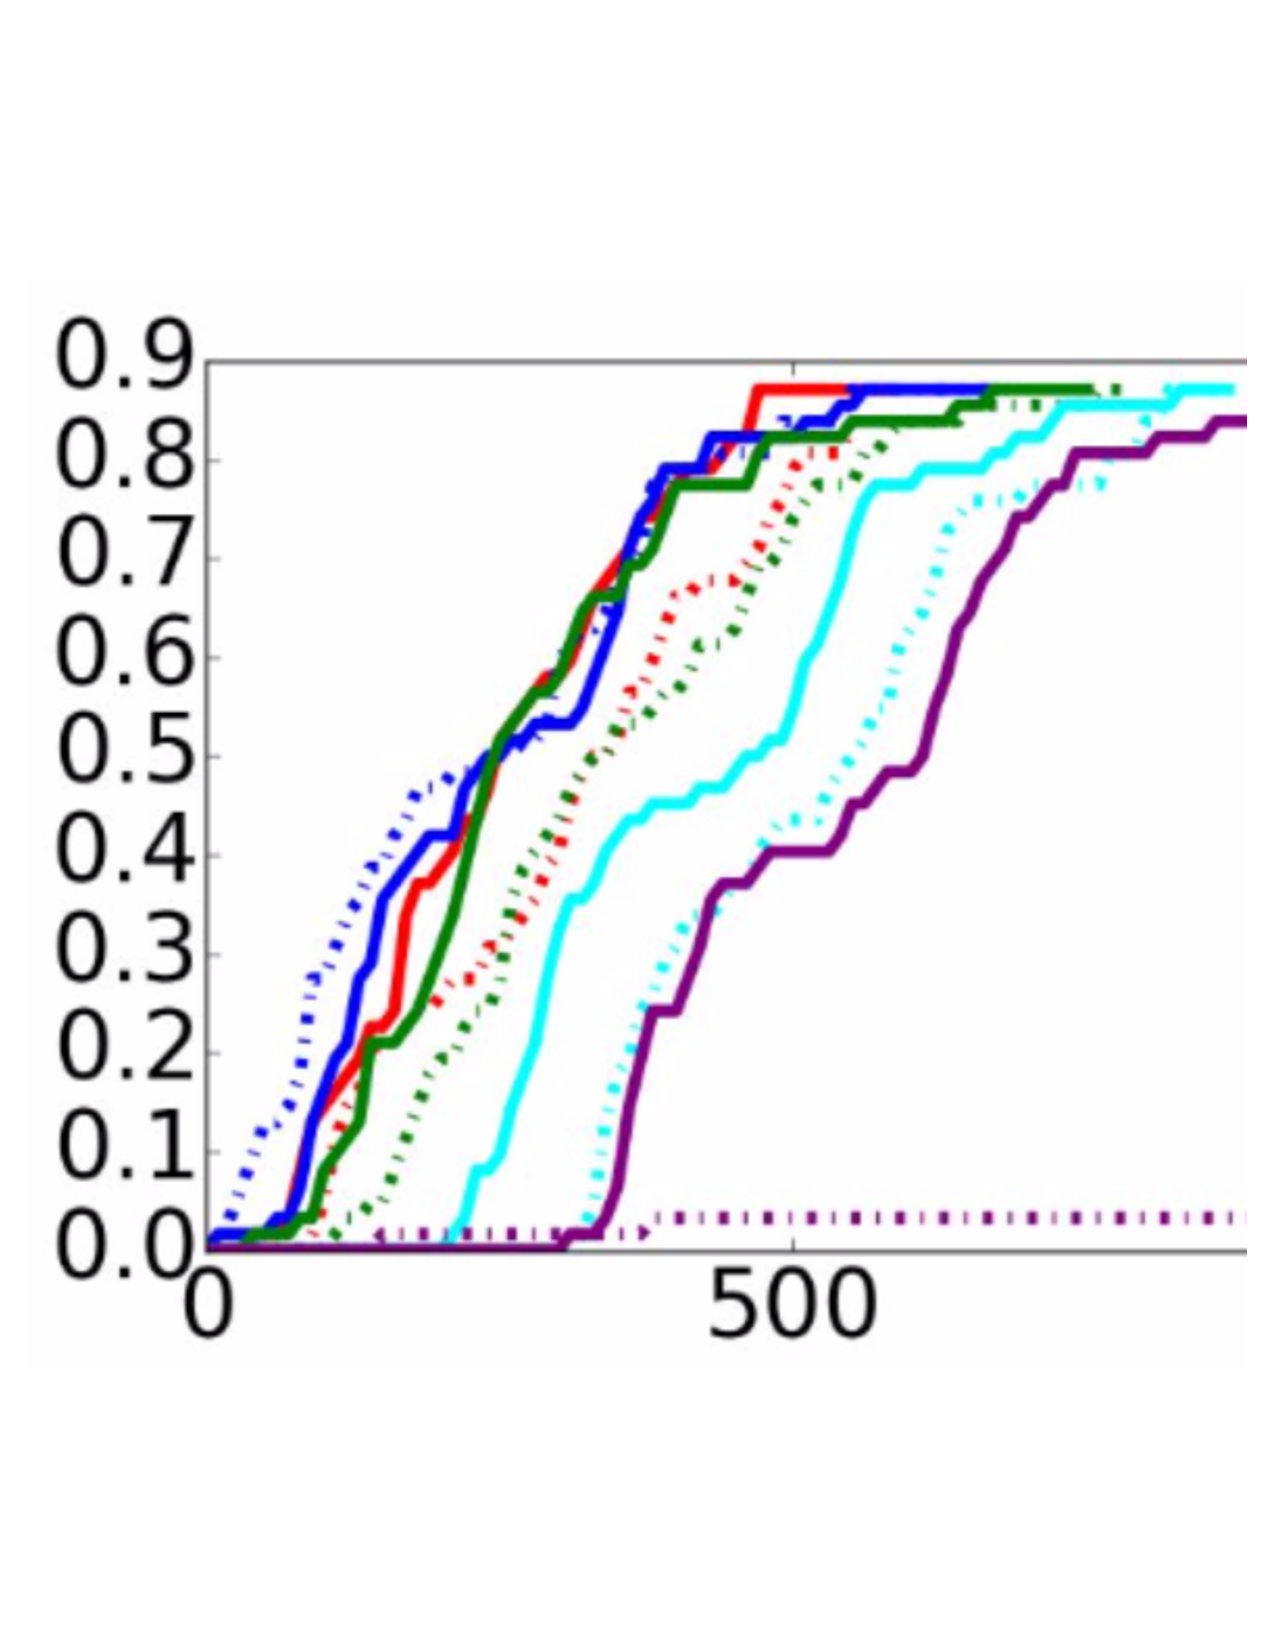
\includegraphics[width=1.4in]{fig/growth.pdf}
% \caption{Characteristic growth curves of \#failed
% tests vs \#test executions (with active learning).}\label{fig:growth}
% \end{wrapfigure} If we can improve test case prioritization, then this
% would have three specific and very useful advantages.
% Firstly,  {\em faster testing}.
% If we can improve test case prioritization with the our active learning methods (the E2 method of \tbl{algorithms} and \fig{relative}), then     we can 
% stop   testing sooner, and also
% know how many bugs are left to find.
% The  test growth curves have a characteristic shape (see \fig{growth}).
% By fitting a parametric  equation to these curves, we can extrapolate forward to infer
% how many more failures will ever be found by the current tests. Using that knowledge,
% developers can then make informed decisions about the cost-effectiveness of futher testing. For example, in \fig{relative}, the E2 method performed so well
% since it terminated when its curve extrapolations reported that it had found 95\% of all failing tests.



% Secondly,  {\em more versions of the software,
% written faster}.
% Consider the case where a full test suite takes hours (or days) to run
% but, using our {\bf strategies}, we can find failing tests in just a few
% minutes to hours. 
% In that case, the testing can be halted early so the   developers build  a 
% new (and fixed)   version.

% Thirdly, {\em cheaper  testing that steals fewer resources from other tasks}.
% Consider the case where a full test suite takes days  (or weeks) to run.
% Such long test runs typically use some commercial 
% cloud or government funded supercomputer resource.
% If we can stop tests early, then developers can spend less money on cloud
% compute facilities. Also, those developers might also be  able to move their tests off
% the supercomputer, thus freeing up that resource for core research.
 

\subsubsection{Endeavoring to Avoid Spurious Warnings}\label{tion:falsealarm}


There exists a bewildering number of   ``rules of thumb'' 
that warning developers about potential problems with software.
For example,
Riel~\cite{riel1996object} lists 61  rules such as ``beware of many accessors''~\footnote{Beware  classes that have many accesser  methods defined in their public interface, many of them imply that related data and behavior are not being kept in one place.}. 
Also, 
Fowler et al.~\cite{fowler99}
offers  a list of ``code smells'' such as ``beware shotgun surgery''\footnote{Making any modifications requires that you make many small changes to many different classes.}. 
Many of these warning rules
have been coded up into automatic agents that can review  a very large code base.
For example, the FindBugs   tool~\cite{Ayewah08} warns  developers to over 400 potential problems such as ``Empty finalizer should be deleted'' and `` Class defines equals() but not hashCode()''.

 The problem with these  tools is  {\em excessive
spurious warnings} that require much time to read, assess, then change the associated
code.
This is a major problem.
Johnson et al. \cite{johnson2013don} investigated why developers are not widely using static analysis tools. They conducted reviews with 20 developers
and found that false positives, and the way in which the warnings
are presented are the main barriers. 
Worse still,   not all relevant warnings are worth fixing.
PI Menzies, with his graduate student Rahul Krishna have shown that the majority
  changes proposed by (e.g.) Fowler's bad smell list have zero
  impact on code quality~\cite{KrishnaML16}.



  
  
  Avoiding spurious warnings is a major problem that has been
  studied by
  many researchers~\cite{hanam2014finding, heckman2008establishing, heckman2009model, kim2007prioritizing, kim2007warnings, kremenek2004correlation,liang2010automatic, ruthruff2008predicting,shen2011efindbugs,
yuksel2013automated}. For example 
Heckman and Williams~\cite{heckman2009model}
conducted a systematic literature
review of actionable warning identification techniques. They identified 21 studies and analyzed the identification approaches, the
evaluation methodology, subject projects, etc. Allier et al.~\cite{allier2012framework} proposed a framework to compare six error ranking algorithms and
identified the best algorithms to rank warnings. 
Avgustinov et al. \cite{avgustinov2015tracking} presented
an approach to track static analysis warnings over the history of
a project, and further use the information to capture developer's
characteristics.  
%Thung et al. \cite{thung2015extent} studied to what extent could field defects
%be detected by the state-of-the-art static analysis tools.

 The above research is commendable in many respects. But, repeating the main theme of this proposal, it is an open question if these methods
from standard empirical SE applies to computational science software.  The methods in the above paragraph were mostly manual studies requiring
a daunting amount of effort to repeat across (e.g.) the sample systems of \tbl{samples}.





 Happily, there is a better, faster, way to tune warning messages
to computational science software. Using the active learner of Figure~2, it is possible for developers  to review just a few  warning messages (marking them ``relevant'' and ''ingore'').
PI Menzies and his graduate student
Xueqi Yang tested this approach (but not on computational
science code). As seen in \fig{warn}, after reading
 10\% of the warnings, a developer has found 80\% of the warnings they would take act on. Better yet, 
this active learner generates
a classifier that could  automatically review the rest
of the warnings, deleting the irrelevant ones.


The case study of \fig{warn} comes from an open source JAVA system;
i.e. {\em not} computational science software. It remains to be seen if this approach is effective for computational science. 
Hence, we propose,
adding   our warning active learning {\bf strategies}
to {\IT}; then
applying them  to warning messages  generated  from \tbl{samples}, and 
{\bf tuning}  as necessary.


\begin{figure}  
\fbox{%
\begin{minipage}{2.7in}
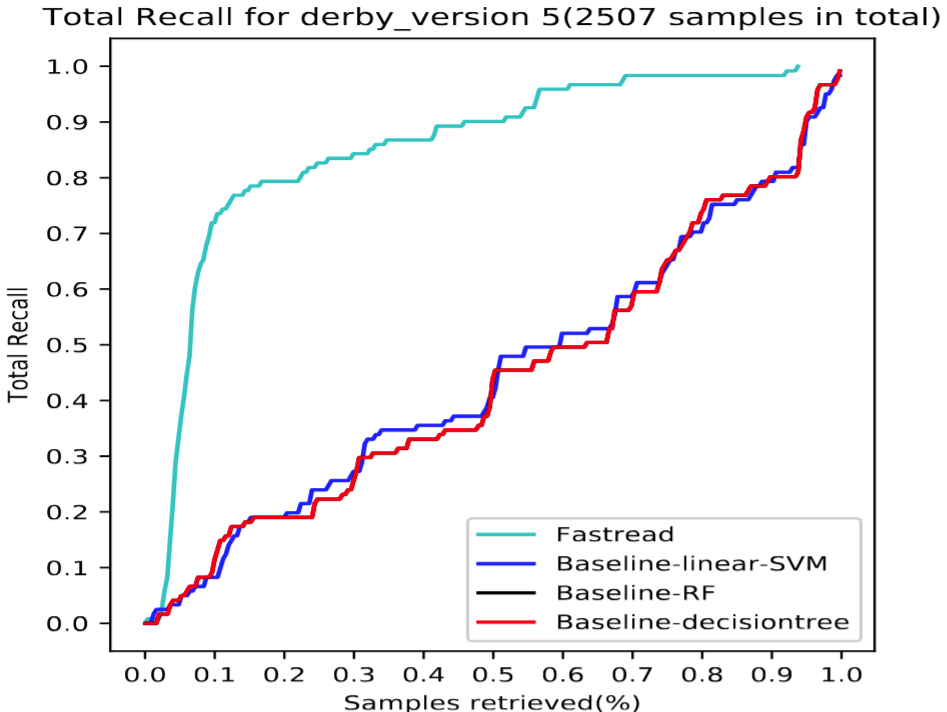
\includegraphics[height=2.2in]{fig/test4.PNG}
\end{minipage}~\begin{minipage}{3.7in}
{
\bi
\item
X-axis shows all warnings.
\item
Y-axis {\bf yield}
 shows percent of ``relevant'' warnings
 discovered so far  (where ``relevant'' means ``a developer will take action on this warning'').  \item
 Top line
 shows  our preferred active learning {\bf strategy}.
 Note that this is the same active learner as used in ~~~ Figure~2.
 \item
 Other lines shows results from other, inferior,  warning prioritization
  {\bf strategies}.from  the literature. 
 \ei}
 \end{minipage}}
 \caption{ Active learning results for learning a classifier for relevant warning messages.} \label{fig:warn}
 \end{figure} 
%for computational science, their results need to be checke for comtpuational science projects.
% Fristly, most of the above are most manual methods that take much effort to complete. H

% Then, we applied our approach to the 446 projects
% seen in six open source effort datasets collected and developed by Qi et al.~\cite{QiEffort17} from Github. In Qi et al.'s work, they implemented a platform for GitHub data crawling and filtering, and extracting necessary information for effort estimation tasks. They also propose a specific algorithm to make the collected dataset have dynamic expansion capability~\cite{QiEffort17}. Using the data sets from Qi et al., we can validate our approach's effectiveness in recent software effort estimating tasks. For the details about these newly collected datasets, see Table~\ref{table:dataset}.



\begin{figure}[!b]
\begin{center}
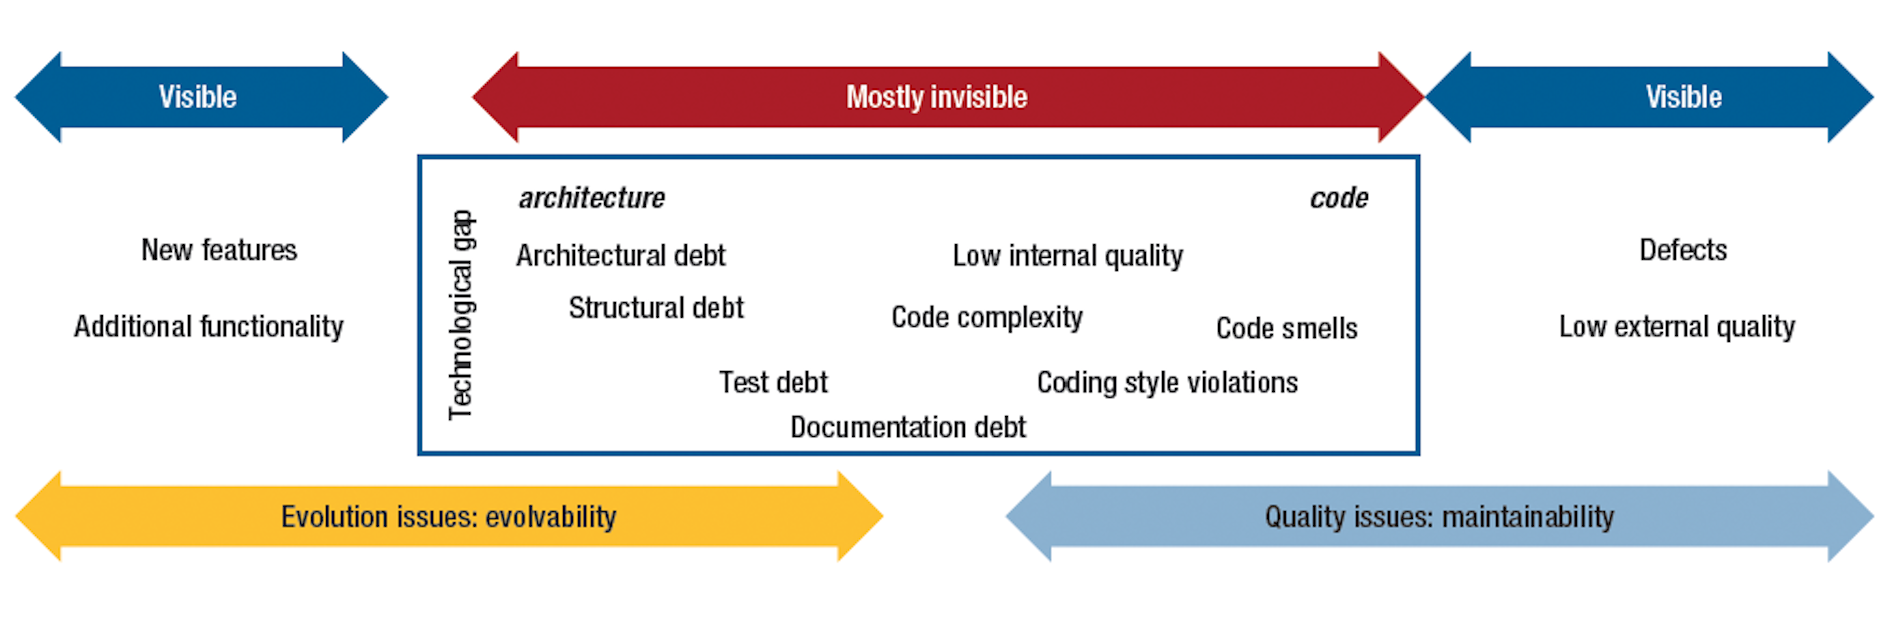
\includegraphics[width=6in]{fig/debt.png}
\end{center}
\vspace{-7mm}
\caption{Impact of technical debt on software. From~\cite{Ozkaya12}.}\label{fig:debt}
\vspace{-2mm}
\end{figure}


\subsubsection{Endeavoring to Avoid Technical Debt}\label{tion:effort}
When developers cut corners and make haste to rush out code, then that code
often contains {\em technical debt}; i.e. decisions that must be repaid, later on, with further work.
Technical debt is seen in (e.g.) bad architectural decisions
such as not
separating the computational core of the code from the interface components. 


Technical debt is like dirt in the gears of software production.
As it accumulates,   development becomes harder and slower. To continue the above example,  if the core and the interface are not properly separated, then it can be hard to port the code to new platform (e.g. to make it a web-service).  
\fig{debt} lists other other areas  adversely effected by technical debt including {\em evolvability} (how fast we can add new functionality) and {\em maintainability} (how well we can keep bugs out of the code). {\IT} aims to tackle thi problem in two aspects---identifying existing technical debt and avoiding future    technical debt.


\textbf{Identifying Existing Technical Debt:} Technical debt is often self-admitted by the developer in code comments\cite{potdar2014exploratory}. This is called Self-Admitted Technical Debt (SATD), where the developer mentions about the debt that he or she is leaving behind for future reference in the source code comments 
``{\em hack, fixme, is problematic, this isn't very solid, probably a bug, hope everything will work, fix this crap}''. Therefore the SATD can be identified by asking a human to read through the source code comments. Since this is a tedious, time consuming and error-prone process, SE researchers have tried various ways to find SATDs faster, with less effort~\cite{maldonado2015detecting,maldonado2017using,huang2018identifying}. As shown in Figure~\ref{tab:SATD}, these studies suggest that supervised learning models trained on SATD comments from other software project can be applied to predict for SATD comments in a new software project, thus saving human efforts for reading the comments.


\begin{wrapfigure}{r}{3in}
\small
\begin{center}
\begin{tabular}{l|ccc}
Software Project & Precision & Recall & F1-score \\\hline
ArgoUML          & 0.80     & 0.85  & 0.83    \\
Columba          & 0.77      & 0.84  & 0.80    \\
Hibernate        & 0.83     & 0.75  & 0.79    \\
jEdit            & 0.70     & 0.41   & 0.52    \\
JFreeChart       & 0.61     & 0.79  & 0.69    \\
Jmeter           & 0.80     & 0.77  & 0.78    \\
JRuby            & 0.83     & 0.86  & 0.84    \\
Squirrel         & 0.708     & 0.602  & 0.651    \\
\rowcolor{blue!10}Average          & 0.756     & 0.733  & 0.737    
\end{tabular}
\end{center}
\caption{Classifying Self-Admitted Technical Debt with Supervised Learning~\cite{huang2018identifying}}
\label{tab:SATD}\label{tbl:SATD}
\vspace{-5mm}
\end{wrapfigure}

\textbf{Avoiding Future Technical Debt:} Another way to mitigate   technical
debt is to remove the conditions under which it first appears.
Many authors agree that the major cause of technical debt is {\em schedule pressure}~\cite{Ozkaya12}.
So,  to test if  software  is threatened by technical debt,
we must ask  ``did/are enough developers working on the code?''.
New results~\cite{Robles:2014,QiEffort17,xia19} show that we can now check
 if there are 
suspiciously too few (or too many) developers
working on a project.
  One interesting feature of this new approach is that it bases its estimates on code attributes drawn from Github repositories. That is, this
  preemptive methods for avoiding
  technical debt might be applicable to computational science software such as those systems listed in \tbl{samples}.


\begin{figure}[!b]
\fbox{%
\begin{minipage}{2.8in}

\includegraphics[width=3in]{fig/header.png}
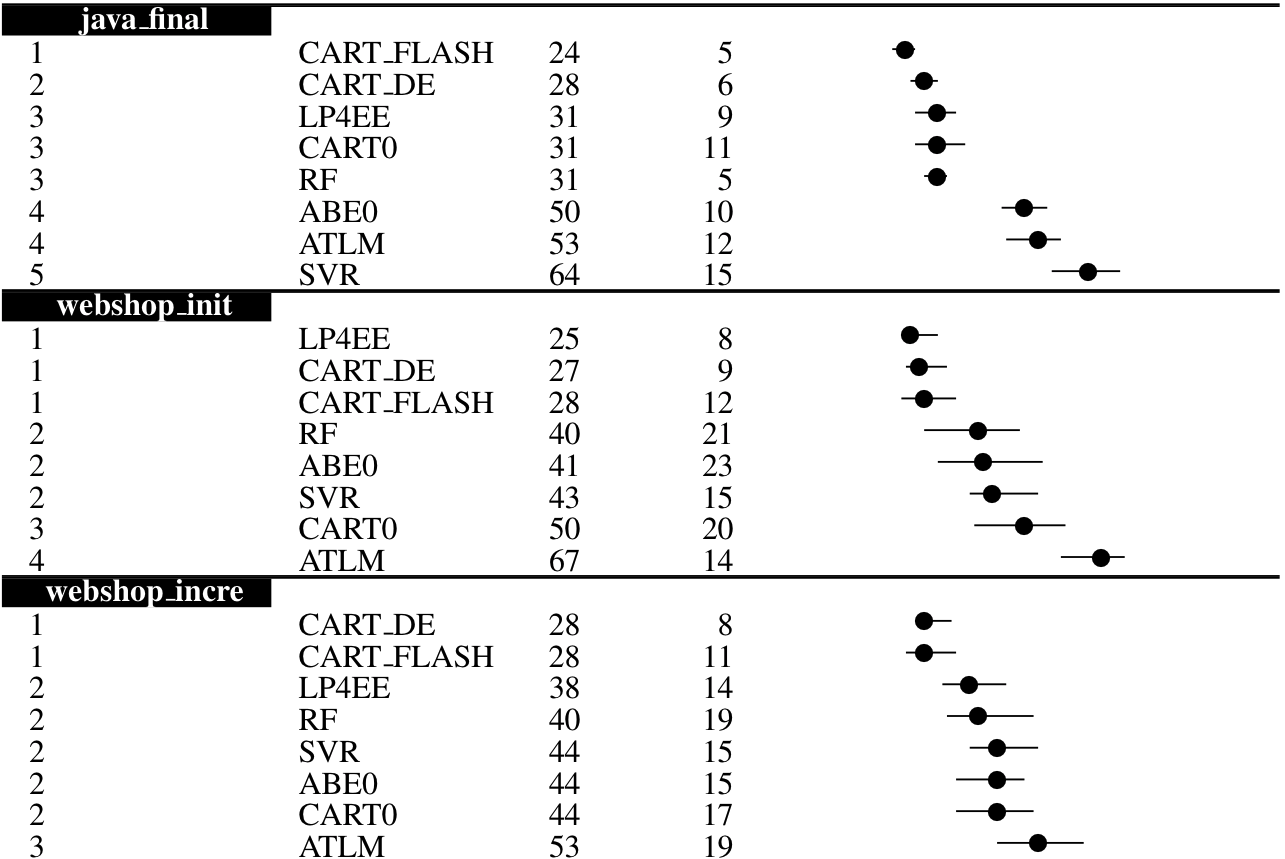
\includegraphics[width=3in]{fig/effort.png}
\end{minipage}~~~\begin{minipage}{3.5in}
{\small
\bi
\item
The  left-hand {\em Rank}
column  groups     results  whose {\bf yields}   are  not  statistically  different  (as  judged  by  a 95\% significance test and an effect size test).
\item
 {\em Method} lists the   {\bf instruments} used for prediction: the CART regression tree learner,  linear optimization using LP4EE;  a random forest (RF) of regression trees);
an analogy-based  method
called ABE), and the   SVR support vector regression method that  uses kernel functions to project
 data to a new hyperspace where  non-linear patterns
are represented in a simpler manner.
\item
The suffix ``\_DE'' or \mbox{``\_FLASH''} denotes an {\bf instrument} {\bf tuned} by a hyperparameter optimizer.
\ei}
\end{minipage}
}

 \caption{ {\bf Instruments} for effort estimation applied to three Github-based JAVA projects.
 Here, the {\bf Yield} is measured in \mbox{{\em (actual - predicted)/actual}} (so {\em smaller} values are {\em better}.} \label{fig:effort}
 \end{figure} 
 For this preemptive method to work, we need to be able to know 
 what are the expected number of developers required
 for a project.
 Recent work, including research by PI Menzies and his graduate student
Tianpei Xia, shows how that expectation can be inferred~\cite{Robles:2014,QiEffort17,xia19}.
 \fig{effort} shows 20 repeated estimation experiments in learning
 the expected number of developers.   That figure shows the error between
 the estimated and actual numbers of developers.
For this proposal, there are several important features of   \fig{effort}:
\bi
\item
In multiple data sets, our best  {\bf instruments} have error
estimates of (24,25,28\%). While that is far less precise than (e.g.) measurements of the speed of light (299,792.458 $\frac{m}{s}$), such an estimator is certainly good enough for detecting if a project is under-staffed and hence in danger of technical debt.
\item
Different projects in \fig{effort} used different {\em instruments} 
to {\em yield} best estimates. That is, like our Figure~2 results, we cannot assume that one standard  {\bf instrument} will suffice for different projects. 
\item 
All the {\em rank=1} error estimators include at least one {\bf instrument} that has been {\bf tuned} by a hyperparameter  optimizer. That is, PI Menzies   already has the
technology that checks if empirical SE {\em instruments} can be successfully {\bf tuned} to computational science (in this case, {\bf instruments} that   recognize suspicious levels of staffing and, hence,   will  suffer technical debt).
\ei
However, just to repeat the main theme of this proposal,
it is an open question if the empirical SE methods used to generate results like \tbl{SATD} and
\fig{effort} can be applied to computational science projects. Nor is is known
if our current {\em tuning} methods for estimation {\bf instruments}
are sufficient to recognize projects prone to
technical debt in computational science projects.

Hence, we propose adding all the {\bf tuning} and estimation {\bf instruments} of  \tbl{SATD} and \fig{effort} to {\IT}, then testing   them on the data of \tbl{samples}
(and adjusting the {\bf tuning} methods, if necessary).
 


% In the $21^{st}$ century, in the age of agile programming\footnote{Traditionally, software developed using a {\em waterfall model}~\cite{Royce:1987} where requirements are written and frozen before the coding.
% This proved to be cumbersome approach, especially
% for code being prototyped to explore
% new ideas (which is a common task for scientific
% software). This century, the watermodel
% is usually deprecated for an 
% {\em agile model}~\cite{fowler2001agile}
% where there exists a continually changing set of desired requirements which developers regularly re-prioritize
% before implementing
% the most valuable requirement next.
% } the test problem grew worse.
% In the agile world, the code
% is continually changing and the challenge is to
% keep the tests up-to-date with the software.
% Agile advocates of ``test-driven development''~\cite{beck2003test}
% proposed writing the test case {\em first},
% then building just enough code to get that test to pass. This principle became so popular that it ended up swamping the development process. Between January and October 2013, Google ran three billion unit tests. Maintaining this test code became more effort that maintaining the code itself. Worse still, the
% time required to run this massive  test suite was over two calendar weeks (even with all Google's superior hardware support)~\cite{Elbaum:2014,}.

% Given this pressure from the agile community,
% the nature of testing has changed. Given test suites take so long to run, the issue is now less of ``how to find all bugs'' but instead ``how to reduce the time required to get some feedback on the bugs in the code''. To that end, 

% The testing problem grew worse
% Later on, in the age of agile programming,
% the nature of the testing problem changed.
% Since testing 
% as test methods grew complex and test suites grew longer to run, it was no longer possible to instantly assess code. Rather, it could take hours to days to weeks to (e.g.) build the formal models needed to run (e.g.) the automatic verification tools to assess software. And even then, the conclusion were only as tate that not bugs were found which is a very different to sayng that no more bugs could be found.

 

%\subsection{Endeavoring to Estimate Development Effort}\label{tion:effort}  

%\subsection{Endeavoring to Avoid Spurious Warnings}\label{tion:falsealarm}


% These claims are based on some initial work funded as part of an EAGER grant.
% The rest of this section discusses the technical details
% required to (a) test these claims using more data from the computational  science community;
% (b) then use the insights from that process to propose innovative methods for helping computational scientists build and maintain better software using fewer resources.



% beck2003test

% technoiiques appy elshewere

% results of Figure~2 were achieved using such simple goal-aware discretizers.
% details: explore all the current projects and not just the 11 explored in\fig{refgreen}.  and more besides
% It turns out that programmers
% hyperparamter optimization

% active elarning

% \subsection{Science and Engineering challenges}
% Computational science   explores natural phenomena 
% at both very large scale (e.g. hurricanes) and very small scale
% using (e.g.) micro-level finite elements analysis. Such software is applied to 
% astronomy, 
% astrophysics, 
% chemistry, 
% climate+weather prediction, 
% economics, 
% genomics, 
% molecular biology, 
% oceanography,
% physics, 
% political science, 
% and many fields of engineering.

% In response to current NSF programmatic areas of interesting, this proposal offers data engineering
% software that   apply automated
% empirical software engineering (SE)
% methods to  computational science projects that make extensive use of software. The proposed {\IT}
% workbench\footnote{ Short for 
% \underline{S}oftware \underline{E}ngineering \underline{N}ow 
% \udnerline{T}ackles   your code \underline{R}emotel\underline{Y}.}
%  will  sustain progress in the CISE field  by positively impacting the computational community's ability to  create  and maintain   higher quality software. This, in turn, will enable faster and better the software development  that that enables more and better and faster computational science.


% Recent results from  an EAGER ``Empirical SE Methods for Computational Software''
% suggest both an opportunity and a challenge for the computational science community.
% PI Menzies found that standard empirical software engineering (SE) methods:
% \bi
% \item Fail badly on computational science software, if used in the standard ``off-the-shelf'' manner;
% \item But succeed very well if those standard methods are tuned to the particulars of computational
% science (specifically, as discussed below, if those methods are tuned to
% the language used by computational  scientists to describe ``defects'').
% \ei
% This result leads to the conjecture that many other empirical SE methods {\em might} be suitable for
% computational science, but only if those methods are first especially adapted to the domain
% of computational science.

% This proposal tests that conjecture.  If successfully, then a large number of automatic quality
% agents could be applied to numerous computational science software. This, in turn, would lead
% to better and faster creation of maintenance of the software needed to 
% support the computational science ecosystem.
 



\section{Management Plan}\label{tion:plan}

The previous section described ``what''  {\bf yields} we can collect from  different {\bf endeavors}.
This section describes ``how'' we will use those {\bf yields}, plus some other metrics,
to explore  Claims 1,2,3,4,5 from \tion{intro}.

In the following:
\bi
\item
  The metrics \#2,4,7,8,9 (described below)  address the claims listed in \tion{intro} while the
 other metrics address   specific requirements
of the CSSI solicitation.
\item
Most of the following metrics are qualitative in nature. The exception is Metric \#8
which will allow a rigorous statistical test of the value of {\IT}. For more on those tests,
see the discussion on {\bf Claim5} at the end of \tion{other}. \ei
\noindent
\subsection{Architecture}   {\IT} will be written in JAVA/Python and 
combine tools from several existing open source toolkits such as 
Scikit-Learn~\cite{scikit-learn}, jMETAL~\cite{durillo2011jmetal}, and Commit.Guru~\cite{commitguru}.
To that suite of software we will add tools recently developed in PI Menzies's lab including
the data processors of Agrawal etl'18~\cite{agrawal2017better}; 
the FLASH hyperparameter  optimizer~\cite{nair2017flash};
the FASTERAD active learner~\cite{Yu:2018,Yu2019}; as well as code
from several other prototoypes (all the code used to generate the    Figure~2 result;
the test prioritization methods tested in \fig{relative};  
the warning analyzer used in    \fig{warn};  
and the technical debt analysis tools used in \tbl{SATD},
\fig{warn}~\cite{xia19}). Further, as the research in our lab continues,
we foresee that other, newer, tools will also be added to {\IT}.





{\IT} will also contain data files holding all the features we extracted from \tbl{samples}. This is useful
since it will allow other researchers to quickly repeat/improve/refute our results without having
to first perform tedious web-scale data collection.

{\IT} will also contain the source core required to reproduce 
our proof-of-concept papers (discussed below). For example, if  a  paper
has research questions RQ1, RQ2, then our code will come with shell scripts
 RQ1.sh, RQ2.sh etc that store the code we executed to answer the research questions.


\subsection{Adaptability to New Technologies} Toolkits like Scikit-Learn and jMETAL
  are currently the international distribution method
for new data mining and optimization
algorithms. Hence, whenever Scikit-learn or jMETAL changes, {\IT} will be positioned to access
and use the  latest innovations  

\subsection{Adaptability to Changing Requirements}
As stated above, this proposal will use {\IT} to explore the four {\bf endeavors}
described above as well as  other tasks as time and opportunity permits and as requested by computational scientists.
We will maintain a roadmap document so that if (for pragmatic reasons)
we cannot currently explore a particular new requirement,
our users will know when they can expect that new functionality.


\subsection{Delivery and Outreach Mechanism}\label{tion:outreach}  {\IT} will
be licensed
open source and
stored in a public
 repository
 that anyone can download and run on their own machines. When executed, these tools
can automatically  work through on-line data from computational science projects.  


{\IT}
will be delivered using Github (i.e. using the
{\tt git clone} command)\footnote{If possible, we will also offer Docker files to distribute our system.
That said, the practicality
of that proposal has to be assessed further once we know the size of the shared data sections
in {\IT}.}. 

We anticipate  that {\IT} will need no proprietary licensed products. Hence  {\IT}
will cost \$0.


As to outreach,
 we would work with the organizers of the annual $SI^2$ PI meeting to arrange focus groups at that meeting
 (so we can have detailed  interaction with interested developers).
In-between the $SI^2$ PI meetings, we would also 
run tutorials on our tools (and related concepts in Empirical SE)
at the PEARC conference (one per year)
as well as webinars
for XSEDE  
and the Sciences Gateways series (whenever we have anything interesting to report).
Accordingly, we will log and report:
\bi
\item {\em METRIC0: Number of tutorials given on this material.}
\ei

\subsection{Timeline}
In the first few months of the project, in order to quickly obtain more initial results (which we can use to popularize this project
and raise its profile in the computational science community), we will apply {\IT} to extend the case study of Figure~2, using the rest of the projects in \tbl{samples}.
After that, for the first two years of this work we will spend six months on each
of the endeavors (a)(b)(c)(d) listed in \tion{ende}. 
For the third year, we will look over our tools to see what can be generalized, improved, simplified. This will lead to a code re-organization.
Apart from that, in all years:
\bi
\item
We will not have releases {\em per se} but a continuous integration
of development and code, ready to be used.
To that end, {\IT}
will be stored open source and on-line to be freely available during+after
this proposal. That is,  just as soon as our tools get useful, they will be
available to the general computational science community.
\item
We will use {\IT} to generate numerous proof-of-concept reports;
i.e. two to four research publications per year, ideally
at top-ranked values.
These proof-of-concept papers would be our reports on what happens when we applied 
empirical SE methods to computational science projects. 
\ei
Accordingly we will log and report:
\bi
\item {\em METRIC1: Number of written/published proof-of-concept papers.}
\ei
\subsection{Reproduciblility }
 As stated above,
all our proof-of-concept papers will come with on-line replication packages
with scripts labelled RQ1.sh, RQ2.sh etc that store the code we executed to answer the research questions
of those papers. 


\subsection{Testing and Documentation}
The proof-of-concept reports will be the
systems-level tests of {\IT}.
As to documentation, we   commit to  maintaining  the standard of documentation proposed
in the Code Carpentry  paper {\em Good Enough Practices for Scientific Computing}~\cite{Wilson16} which include an {\tt INSTALL.md} files describing downloading
an installation plus {\tt README.md} files describe example usages of the system.
As to other documentation, we will use a literate  programming style of documentation; i.e.
or Jupyter notebooks;  
 code and classes docs generated  from  code,
presented in a public  {\tt /docs} directory in
our repos.



\subsection{User Interactions} We would create a simple on-line registration Google
form  where interested developers can register their repository with us. Accordingly, we will log and report: 
\bi
\item {\em METRIC2: How many projects register themselves for our service.}
\ei
Our agents will then analyze the 
registered projects using our automatic agents,
posting   issue reports back to those repositories.
Accordingly, we will log and report: 
\bi
\item {\em METRIC3: Number of projects analyzed.}
\ei
We will  track if those issues
are ever acted on by  projects (and if none are, then that would indicate our tools are reporting
irrelevancies). Accordingly, we will log and report: 
\bi
\item {\em METRIC4: How computational scientists change their projects
in response to our recommendations.}
\ei
As to day-to-day support of teams using our tools,
some of  their time will be dedicated
to offering   support and advice to  those computational science teams.
Accordingly, we will log and report
\bi
\item {\em METRIC5: Number of help requests from how many projects (trying to run our tools on their code).}
\ei
Since our code will be on-line in a web-accessible repository, we will also be able
to gauge the community's interest in our work via the number of pull requests and issue
or
bug reports posted to our repository:
\bi
\item {\em METRIC6: Number of pull requests and issue or bug reports.}
\ei
\subsection{Security} 
We do not anticipate security issues for this project since we will using data that the projects are already placing on-line.

 
 
\subsection{Other Metrics}\label{tion:other}
The above Metrics \#2,4,5,6 (as well as some that follow)  measure
user involvement in this project. They also let us see to what extent
users accept our new tools.

The rest of this section discusses the metrics required
to explore  the
five claims of \tion{intro}.   

To  explore   {\bf Claim1 = relevance}, we must try
to interest   computational scientists in our methods.
For that task, we will use the above mentioned
Metrics \#2,4.    That is to say, we will use computational scientist to judge if what we are doing
is worthwhile.  Note that we all ready have some preliminary indications that we may do well
according to Metric \#2 (see the 11 letters collaboration attached to this proposal).

Given the wide ranging nature of this
proposal, it may not be true that all our future
work as simple as seen in the Figure~2 case study.
Therefore, to explore  {\bf Claim2 = operational} we must log and report:
\bi
\item {\em METRIC7: The human effort
 required to apply the SE {\bf instrument}.} 
\ei
Metric \#7 will record how hard for humans to  {\bf tune} and {\bf instrument} for computational
science. But are their any benefits justified with respect to  the cost of {\bf tuning}?
To make that assessment, in order to justify,
 \mbox{{\bf Claim3 = must adjust}}, we must log and report:
\bi
\item {\em METRIC8: compare the  performance 
scores {\bf yielded}
using standard empirical SE {\bf instruments}, before and after {\bf tuning}.}
\ei
Note that one unlikely, but very useful result,
would be that the {\bf yield} does not
increase after {\bf tuning}
standard empirical SE methods for computational
science projects. In that case, {\bf Claim3} would be refuted.
Having recorded that possibility, we note that this is very unlikely.
Firstly, the nature of computational science software is very different to the Google- and Facebook- and Microsoft- style of projects used to develop current empirical SE
methods. Secondly, the experience of Figure~2 is that significant adjustments are required
to standard empirical SE methods before they are effective for computational science.

To explore {\bf Claim4 = practical}
we must log and report the effort required to 
adjust SE methods to computational science; specifically:
\bi
\item {\em METRIC9: the CPU time or other platform  costs
required to complete tuning.}
\ei
This metric is subtly different to Metric \#7. In the prior metric, we checked
the difficulty for humans to wrangle together a working system. In this metric we 
measure the cost of the hardware systems (computer hardware,  cloud compute costs, CPU time).
This is an important point since some {\bf tuning}
{\bf strategies}
can be impractically slow~\cite{abs-1807-11112},
particularly if those {\bf strategies} need to be repeated
many times during a rapidly evolving software project.
Worse, if those {\bf strategies} themselves have
to be changed from project to project there we
would be unable to offer any guidelines on how to best
{\bf tune} the next project.

To explore  {\bf Claim5 = valuable}, we would reuse
{\em Metric8} and reflect on the 
  {\em size} of the {\bf yield} difference seen after
  applying empirical SE methods (with or without
  {\bf tuning}, depending on the results of {\bf Claim3}).
  \bi
  \item
  This test would use some statistical significance and
  effect size test (e.g. a 95\% bootstrap sample and Cliff's Delta).
  \ei
  Note that if,
  at the end of the day, empirical SE offers very
  little benefit for computational  science, then we would reject Claim5 and declare
  a negative result from this research.
  
  

%\begin{table}
\caption{Initially,
this proposal will focus on the following
 samples of active computational science projects
(all of which are found in on-line open source repositories). 
{\normalfont Robert Sinkovits (from XSEDE) comments that many of these codes account for the majority of the supercomputer usage in computational
science. While some of these  focus on  computational chemistry,  they   also   include  numerous widely-used support tools (e.g
elasticsearch) or simulation tools that are cross-disciplinary (e.g. the classical simulation tools
used  by molecular biologists).  Also, there are also tools here used in material science (e.g. LAMMPS).
Further, these are just some of the projects found during an initial EAGER-funded projects so, during the three years of
this current proposal, we anticipate that many more projects will be discovered and analyzed by {\IT}.}
}\label{tbl:samples}
{\footnotesize
\begin{center}
\begin{tabular}{r|l@{~}rrr@{~}r@{~}r@{~}rrc}
\renewcommand{\baselinestretch}{0.7}
&   &   &   &   &  &  &   & Analyzed\\  
 & Language & \# Developers & Duration(Years) & \# Commits & \# Stars & \# Issues & \# Releases & in Figure~2\\ 
\hline
BLIS & C & 20 & 4.8 & 1242 & 413 & 142 & 25 &   \\ 
cctools & C	 & 43	& 5.5 & 8881	& 72 & 666 & 159  &   \\
keplerproject & C & 22	& 5.25 & 329 & 26 & 66	& 18 &   \\

\hline
\rowcolor{blue!10}AMBER & C++ & 12 & 4 & 8382 & 32 & 249 & 3 & \checkmark\\
changa & C++ & 19	& 3.5 & 1458 & 13 & 16 & 8 &   \\
cyclus & C++ & 20	& 6.5 & 6579 & 36 & 625	& 47 &   \\
dealii & C++ & 120 & 18 & 41514 & 382 & 1604 & 26 &   \\
GooFit & C++ &	12	& 5.5  & 1508	& 57 & 50	& 12 &   \\
\rowcolor{blue!10}HooMD-blue & C++ & 36 & 2.5 & 9450 & 54 & 330 & 25 & \checkmark \\
irods & C++	& 36 & 5 & 6267 & 236 & 3820 & 34 &   \\
\rowcolor{blue!10}LAMMPS & C++ & 74 & 5.13 & 15814 & 383 & 294 & 91 & \checkmark \\ 
\rowcolor{blue!10}LIBMESH & C++  & 55 & 6 & 17133 & 247 & 449 & 59 & \checkmark \\ 
MADNESS & C++ & 31 & 4.5 & 5193 & 71 & 184 & 3 &   \\
metpy & C++	& 34	& 7.75 & 2199 & 332 & 481 & 20 &   \\
OpenMm & C++ & 38 & 7 & 5838 & 324 & 959 & 22 &   \\
OpenMX & C++ & 11 & 5 & 6993 & 26 & 79 & 62 &   \\
\rowcolor{blue!10}PCMSolver & C++ & 8 & 4 & 1844 & 13 & 88 & 16 & \checkmark \\ 
PLUMED & C++ & 23 & 5.5 & 8075 & 92 & 282 & 35 &   \\
Psi4 & C++ & 79 & 5.5 & 12178 & 247 & 504 &	7 &   \\
SCIRun & C++ & 18	& 6.5 & 8887 & 45 & 1487 &79 &   \\
TRILINOS & C++ & 179 & 3 &	79520 & 310  &	2063 &	141 &   \\\hline
  \rowcolor{blue!10}ABINIT  & Fortran & 23 & 2.3 & 6793 & 53 & 13 & 96 & \checkmark  \\ 
 OpenMolcas & Fortran & 29 & 1 & 565 & 29 & 52 & 2 &   \\ 
MPQC & C++, Fortran & 12 & 5 & 6362 & 28 & 44 & 57 &   \\
NWChem & Fortran & 29 & 1 & 26013 & 70 & 33 & 5 &   \\
OpenMPI & C, Fortran & 147 & 4 &	28680 & 627 & 1424  & 99 &   \\
quantum\_package & Fortran & 11 & 4.5 & 2721 & 18 & 92 & 5 &   \\\hline
elasticsearch & Java & 1103 & 8.5 & 42349 & 37757 & 16918 & 223 &   \\
learnsphere & Java &  9 & 2.5 & 646	& 11 & 34 & 1 &   \\
orca & Java	& 11 & 3.5 & 1103 & 1 & 143	& 19 &   \\
trellis & Java & 3 & 2 & 892 & 26 & 171 & 10 &   \\
\rowcolor{blue!10}Xenon & Java  & 11 & 9 & 2315 & 15 & 378 & 21 & \checkmark \\\hline
abaco & Python 	& 8	& 3.5 & 1112 & 13 & 29 & 7 &   \\
APBS & Python & 19 & 5 & 6642 & 67 & 501 & 8 &   \\
forcebalance & Python &	10 & 5 & 1562 & 48 & 47 &	6 &   \\
foyer & Python & 10 & 3.5 &	343 & 19 &	66 & 8 &   \\
hydroshare & Python	& 30 & 4 &	9387 & 63 & 1708	& 55 &   \\
Luigi & Python & 35 & 6 & 3628 & 10348 & 628	& 37 &   \\
mast & Python & 22	& 5.5 & 5050 & 8 & 471	& 69 &   \\
\rowcolor{blue!10} MDAnalysis & Python & 76 & 3.5 & 5120 & 233 & 1087 & 46 & \checkmark \\
mdtraj & Python	& 45	& 6 & 2971 & 189 & 682	& 21 &   \\
openforcefield & Python &	8	& 1 &1360 & 37	& 70	& 5 &   \\
openmmtools & Python &	10 & 4 &	1156 & 40  & 154	& 31 &   \\
parsl & Python & 11	& 2 & 1268 & 63 & 258	& 15 &   \\
pymatgen & Python & 107	& 7 & 14989	& 322 & 359	& 228 &   \\
pyscf & Python	& 36 & 4.5 & 4666 & 217 & 101	& 41 &   \\
radical-pilot & Python & 17	&  5 & 56900 & 26 & 1269 & 137 &   \\
\rowcolor{blue!10} RMG-Py & Python  & 43 & 1 & 7548 & 112 & 678 & 17 & \checkmark \\
signac & Python	& 8	& 2 & 5000 & 8	& 89 &	5 &   \\
signac-flow & Python &	8 & 2 & 1000 & 5 & 28	&3 &   \\
TauDEM & Python	& 11 & 5.5 & 298 & 102 & 132 & 10 &   \\
Use Galaxy & Python	& 188 & 3.5 & 36005 & 507 & 2269 & 51 &   \\
yank & Python &	8 & 5  &	2728 & 41 & 557 & 34 &   \\
yt & Python & 93 & 1.5 & 23923 & 138 & 1216 & 37 &   \\

\end{tabular}\end{center}}
\label{tbl:summary}
\end{table}
 
%\begin{table*}
\scriptsize
\begin{center}
\caption{Commit labelled  ``worrying'' by 
a keyword method (from Commit.Guru\cite{commitguru})) or   $F^3T$. 
Right-hand side comment comes from a manual inspection.}
\begin{tabular}{l|cc|c}
\renewcommand{\baselinestretch}{0.5}
  \rowcolor{gray!30}               & \multicolumn{2}{|c|}{Label=``worrying?''} & Comment on the\\
 \rowcolor{gray!30} Commit message & Keyword & $F^3T$ &  Keyword labels\\ 
\hline
\texttt{fixed: rmsd\_fit\_trj() failed to write a XTC file} & y & y &   \\ 
\texttt{fixes Issue 143: alignto() now checks that the two selections describe the same atoms} & y &	y &   \\ 
\texttt{Correct bugs due to merge (rhotoxc)}	& y &	y & Correct\\ 
\texttt{Convert tsmear to tphysel in vtorhotf.F90} &	n &	n &  \\ 
\texttt{Universe can load multiple trajectories from positional args} &	n &	n &   \\ \hline
\texttt{NetCDFWriter working (closes Issue 109)}	& n &	y &  \\ 
\texttt{Correction in magnetization rotation (DFPT+PAW)} &	n &	y &  \\
\texttt{Add missing module dependency} &	n &	y & False-Negative\\ 
\texttt{Correct dfptnl\_pert.F90 for parallel computations} &	n &	y &  \\ 
\texttt{Test for issue \#352 now pass} &	n &	y &  \\ \hline
\texttt{documentation updates and fixes} &	y &	n &   \\ 
\texttt{Removed unused expected error from Selections} &	y &	n &   \\ 
\texttt{Test for HOLE changed form error to warning when HOLE binaray is not there} &	y &	n & False-Positive  \\ 
\texttt{Added CHANGELOG entry for fix of Issue \#550.} &	y &	n &  \\ 
\texttt{Make error message clearer in tests for TPR parser} &	y &	n &   \\ \hline
\end{tabular}
\label{tbl:sample}
\end{center} 
\end{table*}
%\begin{table*}[!t]
\small
\centering
\caption{14 independent   features extracted by Commit.Guru \cite{kamei12_jit}.}
\vspace{-10pt}
\label{tbl:metrics}
\resizebox{\linewidth}{!}{
\begin{tabular}{|l|l|l|p{12cm}|}
\hline
\rowcolor{gray!30}Dimension & Name & Definition & Rationale \\\hline
\multirow{5}{*}{Diffusion} & NS & Number of modified subsystems & Changes modifying many subsystems are more likely to be defect-prone \\\cline{2-4}
& ND & Number of modified directories & Changes touching more directories
are more likely to introduce defect. \\\cline{2-4}
& NF & Number of modified Files & Changes touching more files
are more likely to introduce defect. \\\cline{2-4}
& Entropy & Number of modified subsystems & Changes with high entropy are more
likely to introduce technical debt, since a developer will
have to recall and track more scattered changes across
each file. \\\hline
\multirow{3}{*}{Size} & LA & Lines of code added & \multirow{2}{*}{Changes touching more lines of code are more likely to introduce defects.} \\\cline{2-3}
& LD & Lines of code deleted & \\\cline{2-4}
& LT & Lines of code in a file before the changes & The larger the file/module, the more likely that the change would be defective. \\\hline
\multirow{2}{*}{Purpose}  & FIX & Whether the change is bug-fixing? & Changes that fixing the defect are more likely to introduce more defects than changes for new functionality implementation. \\\hline
\multirow{5}{*}{History} & NDEV & Number of developers that changed the modified files & Changed files touched by more developers before are more likely to introduce defects, since different developers have different design thoughts and code styles. \\\cline{2-4}
& AGE & The average time interval between the last and the current change & More recent changes (lower age) contribute more defects than older changes (longer age). \\\cline{2-4} 
& NUC & Number of unique changes to the modified files before & Larger NUC changes are more likely to
introduce defects since a developer will have to recall and track many previous changes. \\\hline
\multirow{5}{*}{Experience} & EXP & Developer experience & The experience of developers has an impact on introducing TD \\\cline{2-4}
& REXP & Recent developer experience & The experience of developers that has often modified the files are less likely to introduce defects (more familiar with the system).  \\\cline{2-4}
& SEXP & Developer experience on a subsystem & Modifications that are made by developer that are familiar with the subsystems are less likely to introduce defects.  \\\cline{1-4}

\end{tabular}} 
\end{table*}

 
 % Before explaining our plan, we note that  
% understanding the literature is not some
% deterministic ``on size fits all'' process. Rather, in our experience, 
% it is an  exploratory process where  analytics 
% struggle to tame some knowledge source by trying
% a range of methods. 
% In order to support such an exploratory process it is important {\em not} to offer
% one tool but rather {\em workflow construction} tools where analysts can mix-and-match between various utilities.  For  a sample of such uitlities,
% see \tbl{overview}.

 
	%\centering
	%\caption{Project Schedule}
	%\label{table-schedule}

 
\newpage\section{Intellectual Merit and Broader Impact}
\label{sec:IM-BI}
\subsection{Intellectual Merit}
This work applies novel active learning and hyperparameter  optimization methods to tasks
that are  central
to the process of software development;
e.g. defect prediction, test case prioritization,
avoiding technical debt, etc.
Also, this work explores how to extend prior standard
SE methods to new kinds of software.
Emprical  SE has been mostly developed for Facebook-, Google- and Microsoft- style software. These three
organizations
are hardly representative of the vast
ranges of  different software types in contemproary practice.  The methods of this proposal 
 could be used to better adapt empirical SE to any other fields of endeavor.


 

\subsection{Broader Impact:} 
We focus on an issue of tremendous economic importance- the creation of better quality software which in turn will be used to find new state-of-the-art research results
in astronomy, astrophysics,chemistry, weather prediction, economics,  genomics,  molecular   biology,    oceanography, physics,  political  science,  and many engineering fields.
For industrial and academic sectors, this work will accelerate global innovations by improving quality and quantity of computational scientific studies.

The PI   teaches senior-level and graduate-level empirical SE, and data  mining classes (and in those data mining classes, all the case studies come from software  engineering). All of the technology developed in this proposal will become case study material for those subjects.  
 
PI Menzies will continue his established tradition of graduating research students for historically under-represented groups. This work will inform the curriculum of  the various NC State  NSF-funded REUs (research experience for undergraduates)
In that program, places are reserved for students from traditionally under-represented areas; e.g. economically challenged regions of the state of North Carolina) and/or students from universities lacking advanced research facilities. While some of the concepts of this grant would be too advanced for that group, some of the simpler concepts and case studies would be suitable for lectures.
  

% \paragraph{7.3. Integration of Teaching and Research}
% Much of the research in this project will also be integrated into a
% classroom environment.  The PI teaches senior-level and graduate-level
% SE, and software analytics   classes (and in those data mining
% classes, all the case studies come from software engineering). All of
% the technology developed in this proposal will become study
% material for those subjects.  Replication studies are especially ripe
% for classroom projects.  Also, through our publications and conference
% work, we would publicize these tools as widely as possible with the
% intent of supporting a broader community working with this approach.

% \paragraph{7.4 Participation of Underrepresented
%   Groups} The PI will continue their established tradition of
% graduating research students for historically under-represented
% groups.  PI Menzies' last two Ph.D. students were an African-American
% women and a gentleman from an economically disadvantaged region
% in central Pennsylvania.  Also, each summer, the PI's department runs an NSF-funded REU
%  (research experience for undergraduates)
% on the ``Science of Software''.
%  At this
% program, places are reserved for students from traditionally
% under-represented areas (e.g. economically challenged regions of the
% state of North Carolina) and/or students from universities
% lacking advanced research  facilities.
% Some of the simpler data mining concepts for this proposal would be suitable for lectures and REU projects.



%\input{f/under}
\subsection{Dissemination of Knowledge}
As described above in \tion{plan} (and, in particular, \tion{outreach}) much of the effort
of this proposal is devoted to reaching out to
the computational science community and including them
in the usage and evolution of {\IT}. 
Apart from that, the PI has  an extensive track record of publishing at senior SE venues and so, it should be expected that the results of this work will be widely visible.

Moreover, the PI has a long history of publishing papers along with reproduction packages holding the data and the scripts required to replicated the papers' results. 
All the our methods used here will be based around software tools in widespread use (Github, Travis CI, etc). 
We will release all our tools via open source licenses so our results can be readily applicable to researcher or developers using Github, etc. 

 
\section{Prior Results}
\label{sec:PriorResults}



This proposal is the next logical step in the PIs's work on analytics and text mining
{PI Menzies} has worked extensively in that arena.
Most  recently, Co-PI Menzies worked on \underline{(a)}~CCF-1302216, 2013-2107, \$271,553;   \underline{(b)}~``SHF: Medium: Collaborative: Transfer Learning in Software Engineering''. 
\underline{(c)}~The {\bf intellectual merit} of that work was to
define novel methods for sharing data, many of which were the precursor to the methods of this proposal.  That work generated the publications  \underline{(d)}~\cite{krishna2018bellwethers,PetersML15,krishna16,he13,Me17,fu2016tuning,krishna2017learning} concerning prediction and planning methods.
The {\bf broader impact} of that work was to
enable a new kind of open science-- one where all data is routinely shared and is capable of building effective models no matter if it is obfuscated for security proposes.
The methods of this project, while targeted at software engineering, could also be applied to any other data intensive field.   
 \underline{(e)}~Data from that work is now housed at the SEACRAFT publicly accessible repository~\cite{seacraft}. That work  funded two Ph.D.s at NCSU. \underline{(f)}
N/A.  

Another relevant research grant is 
\underline{(a)}~OAC-1826574, 2018-2018, 
\$124,628.00;
\underline{(b)}-
``EAGER: Empirical Software Engineering for Computational Science'';
\underline{(c)}~That work lead to the Figure~2 results
shown in this proposal.
The {\bf intellectual merit} of that work was to
conduct initial explorations into novel methods for adapting SE methods to computational science.
The {\bf broader impact} is the same as this work.
\underline{(d)}~That work generated one conference paper~\cite{abs-1807-11112}
and another journal publication under review publications.
 \underline{(e)}~Data from that work is now housed at the SEACRAFT publicly accessible repository~\cite{seacraft}. That work  funded one Ph.D. at NCSU. 
 \underline{(f)} N/A.  





%There are other grants that could be listed here but as we understand recent changes to NSF grant guidelines, the above are all that is allowed/required.

\end{nsfdescription}

\begin{nsfreferences}
      \bibliography{proposal,zhe,unsuper,sherry,fahmid}
\end{nsfreferences}
%\Facilities{part_facilities_combined}
%\BudgetJustification{University of Alabama}{alabama_budget}
\newpage
%\section*{Facilities}
\begin{Facilities}{North Carolina State University}

\section*{Offices:}
The project PI has
and offices in their   CS Department.  This
department
has adequate space to house all research assistants
working on this project. All offices are wired for high-speed network
access.

The PI's departments at  NC State provide the space and basic networking services to
carry out the experiments, secretarial and administrative support as
well as general-purpose office equipment ({\em e.g.}, fax, photocopiers,
etc.).

\section*{Lab Space}
The PI has their own lab space at   NC State.
PI  Menzies' RAISE lab (Real-World 
AI and SE) is a newly renovated space 
containing over 1,500 ft\textsuperscript{2} of research space and 
15 cubicles, a meeting space, printer, and wide screen projector. 

\section*{Compute Facilities}
Part of {\IT} will involve comparatively assessing different 
technologies.   For that process, it will be useful to have some large scale compute facility.
 
 At NCSU, students working on this grant will have access to  a 108-node compute cluster named ARC with 
2,000 cores (AMD Mangy-Cores), Infiniband QDR interconnect, per node
power monitoring, GPUs and SSDs and parallel file system support,
which was funded by an NSF CRI that he is the main PI of together with
5 co-PIs.  
The ARC facility is providing local and remote researchers with
administrator/root privileges for Computer Science experiments at
medium scale. This allows any of the software layers, including the
operating system and Infiniband switch network routing tables, to be
modified for experimental purposes, e.g., to experiment with different
network topologies.  For large-scale demonstrations, other 
facilities will be utilized (the HPC discussed below.


Additionally, NC State University provides a High-Performance Computing (HPC) facility as a part of the initiative to provide state of the art support for research and academic computing. HPC system (called henry2) provides NC State students and faculty with entry and medium level high-performance research and education computing facilities, consulting support and scientific workflow support. The HPC ecosystem consists of 1233 dual Xeon compute nodes in the henry2 cluster. Each node has two Xeon processors (mix of dual-, quad-, six-, eight-, ten-core, twelve-core) and 2 to 6 GigaBytes of memory per core. The total number of cores increases as more cores are purchased and now exceeds 10000. The nodes all have 64-bit processors. All HPC projects have capability to run jobs using up to 128 processor cores up to 48 hours and smaller jobs up to a week.

%This platform can be used for software development of integrated
%architectures. We plan to experiment on multiple Intel Core i7 x86
%CPU/GPU platforms, AMD APUs, and 2 NVIDIA Tegra TK1 development kits
%in our lab. We also we plan to acquire additional integrated platforms
%as part of this grant, including an Intel Xeon Phi (Knight's Landing).

% \paragraph{Remote Computing Resources:}
% The PI has access to the GPU cluster and Infiniband cluster at the
% Thomas Jefferson National Accelerator Facility of the U.S. Department
% of Energy. The GPU cluster includes 117 Intel Nahalem nodes, equipped
% with over 200 Tesla S1070 in total and connected with QDR or SDR
% Ininiband. The Infiniband cluster contains three sub-clusters. One
% contains 224 nodes, each equipped with dual quad-core 2.53 GHz
% Westmere CPUs, 24 GB memory, and QDR (40 Gb/s) Infiniband; one
% contains 320 nodes, each equipped with dual quad-core 2.4 GHz Nehalem
% CPUs, 24 GB memory, and QDR (40 Gb/s) Infiniband; another contains 392
% nodes, each quipped with dual quad-core 1.9 GHz Opteron CPUs, 8 GB
% memory, and DDR (20 Gb/s) Infiniband.
\end{Facilities}
% \CommunityOutreach{old/nsf_community}
\DataManagementPlan{old/nsf_data}
\ProjectPersonnel{old/nsf_personnel}
% \ProjectRoles{old/nsf_roles}
\end{document}
